\documentclass[journal]{IEEEtran}
\usepackage[T1]{fontenc}
\usepackage{amsmath,amssymb}
\usepackage{graphicx}
\usepackage{url}
\usepackage{booktabs}
\usepackage{array}
\usepackage{tikz}
\usetikzlibrary{positioning,arrows.meta}
\usepackage[hidelinks]{hyperref}
% Figures are read straight from the repository (compile from paper/)
\graphicspath{{../figures/DE/}{../figures/methylation/}{../figures/GENIE3/}{../figures/PANDA/}%
{../figures/LIONESS/}{../figures/ALPACA/}{../figures/validation/}{../figures/other/}%
{../figures/tissue_generality/}{../results/validation/}{../figures/}}
\makeatletter\g@addto@macro{\UrlBreaks}{\do\_\do\-\do\.}\makeatother
\DeclareUrlCommand\repo{\urlstyle{tt}}
\newcommand{\gene}[1]{\textit{#1}}
\newcommand{\twofig}[2]{\includegraphics[width=0.49\columnwidth]{#1}\hfill\includegraphics[width=0.49\columnwidth]{#2}}
\markboth{Preprint}{Preprint}

\begin{document}

\title{Gene Regulatory Network Construction in Fragile X Syndrome:\\
An Integrative Transcriptomic, Epigenomic, and Permutation-Tested Computational Framework Across Two Independent Cohorts}

\author{Aditya~Jha and Softya~Sebastian%
\thanks{A.~Jha and S.~Sebastian are with Vellore Institute of Technology, Chennai, India (e-mail: aditya.jha@vitstudent.ac.in; softya.sebastian@vit.ac.in).}%
\thanks{All code, result tables, figures, run logs and a Google Colab notebook that reproduces the analysis from public data are available at \url{https://github.com/adj-04/fxs-research}. Supplementary items S1--S13 are files in that repository (Table~\ref{tab:supp}).}}

\maketitle

\begin{abstract}
Fragile X syndrome (FXS) arises from CGG-repeat expansion and promoter hypermethylation at \gene{FMR1}, but how this single silencing event reorganizes the wider transcription-factor (TF) regulatory landscape, and whether small patient cohorts can detect such reorganization, is poorly characterized. We built a multi-omics pipeline combining DESeq2 differential expression, cell-composition-adjusted 450K methylation analysis, and GENIE3, PANDA, LIONESS and ALPACA network inference, applied to two independent NCBI-reprocessed RNA-seq cohorts (iPSC-derived cerebral organoids, $n=12$; NPC/B-lymphocyte/iPSC lines, $n=10$) and a peripheral-blood methylation cohort ($n=62$). GENIE3, PANDA and ALPACA statistics were tested against pooled permutation nulls fine-grained enough to permit false-discovery-rate (FDR) control, and LIONESS edges with a timepoint-adjusted linear model. \gene{FMR1} silencing replicated across all three datasets (log$_2$FC $-10.47$ and $-8.91$; $\Delta\beta=0.58$ across 15 promoter probes). Genome-wide, the cohorts did not agree (effect-size $r=0.031$; sign concordance 50.5\%), no GENIE3, PANDA or LIONESS edge survived FDR $<0.05$, and PANDA scores were indistinguishable from a randomized-prior null. Only \gene{FMR1} and \gene{FMR1-AS1} were significant in more than one tissue context. One ALPACA differential module did survive correction (FDR $=0.0099$): five nodes comprising the neurodevelopmental TFs BARHL1 and OTX1 and the neurofilament gene \gene{NEFL}. Among a priori FXS-associated regulators, REST received the most consistent support: it ranked first in ChEA3's ENCODE ChIP-seq library for both its GENIE3- and PANDA-predicted targets, and significant enrichment of its predicted targets among curated targets in TRRUST (FDR $=0.004$) and CollecTRI (FDR $=5\times10^{-6}$). At the sample sizes available for a rare monogenic disorder, network-level inference is best treated as hypothesis-generating; we release the full, reproducible pipeline.
\end{abstract}

\begin{IEEEkeywords}
Fragile X syndrome, gene regulatory network, GENIE3, PANDA, LIONESS, ALPACA, DNA methylation, permutation testing, cross-cohort validation, tissue specificity, reproducibility.
\end{IEEEkeywords}

\section{Introduction}
\IEEEPARstart{F}{ragile} X syndrome (FXS) is the most common inherited cause of intellectual disability and a leading monogenic contributor to autism spectrum disorder~\cite{santoro2012}. It results from expansion of a CGG trinucleotide repeat in the 5$'$ untranslated region of \gene{FMR1}~\cite{peprah2012}, which triggers promoter hypermethylation, transcriptional silencing, and loss of the fragile X messenger ribonucleoprotein (FMRP)---a process linked to broader genome instability at repeat-expansion loci~\cite{hayward2021}. FMRP normally regulates translation and localization of a large set of neuronal mRNAs, so its loss has knock-on effects across synaptic development, neuronal maturation, and cognition.

Prior transcriptomic and epigenetic work has mapped the downstream expression changes tied to \gene{FMR1} silencing in reasonable depth~\cite{li2020,malachowski2023}, and reversing promoter methylation partially restores neuronal phenotypes in patient-derived models~\cite{liu2018,brykczynska2016}. Less attention has gone to how the TF regulatory architecture itself is reorganized once \gene{FMR1} is lost, and to whether that reorganization is detectable with statistical confidence in the small cohorts available for FXS.

We state our contribution precisely. The CGG-repeat $\rightarrow$ promoter-hypermethylation $\rightarrow$ \gene{FMR1}-silencing mechanism is well established~\cite{peprah2012,hayward2021,liu2018,brykczynska2016}, and this paper does not claim to revise it; \gene{FMR1} silencing is reproduced here as an internal validity check on sample labels, processing and cohorts. The contribution is downstream of that mechanism and has two parts: (i) a permutation-tested, cross-cohort-validated framework for asking whether network-level regulatory reorganization after \gene{FMR1} loss is statistically detectable at realistic FXS sample sizes, and (ii) an explicit classification of which downstream transcriptional and methylation changes are shared across tissue contexts and which are specific to one, using the three independently derived tissue sources available (cerebral organoid, NPC/B-lymphocyte/iPSC, peripheral blood) as deliberate probes rather than as a confound. We report both parts in full, including where they are negative.

Differential expression identifies genes whose mean expression changes between groups but does not model how regulatory interactions shift. Gene regulatory network (GRN) inference models TF--target relationships explicitly. GENIE3~\cite{genie3} infers them from expression with tree-based ensemble regression; PANDA~\cite{panda} combines expression with TF-motif and protein--protein interaction (PPI) priors by message passing; LIONESS~\cite{lioness} extends PANDA to sample-specific networks; and ALPACA~\cite{alpaca} detects differential community structure between two networks.

We assemble these four methods into one pipeline for FXS and add three safeguards that matter at small $n$: (i) replication in a second, independently processed RNA-seq cohort; (ii) a permutation null for every network-level statistic, built so that its resolution is fine enough for FDR correction to be possible; and (iii) explicit adjustment for the dominant nuisance variables in each dataset (developmental timepoint in the organoids, donor in the validation lines, leukocyte composition in blood). Fig.~\ref{fig:workflow} summarizes the pipeline:
\begin{enumerate}
\item differential expression in both RNA-seq cohorts (DESeq2), with a donor-blocked sensitivity analysis in the validation cohort;
\item cell-composition-adjusted differential methylation in blood (limma, EpiDISH);
\item GENIE3 inference of TF$\rightarrow$target edges over a label-independent target universe;
\item PANDA networks from JASPAR motifs, STRING PPI and a continuous promoter-methylation accessibility weight;
\item LIONESS sample-specific networks with a per-edge test adjusted for timepoint;
\item ALPACA differential modules;
\item pooled permutation nulls for GENIE3, PANDA and ALPACA;
\item tissue-generality classification across the three tissue contexts;
\item cross-cohort concordance (DEG overlap, effect-size correlation, rank--rank hypergeometric overlap); and
\item in silico validation against ENCODE ChIP-seq, TRRUST and CollecTRI, plus TF-activity inference in both cohorts.
\end{enumerate}
We present this as a template for a rigorously validated and fully reported framework when patient data are, as is usual for a rare monogenic disorder, too few to power network inference on their own.

\section{Related Work}
Malachowski et al.~\cite{malachowski2023} used spatial heterochromatin mapping to show coordinated silencing of long synaptic genes in FXS; an NCBI-reprocessed cohort from that study's raw data forms our validation dataset. Li et al.~\cite{li2020} built molecular interaction networks around FMRP-regulated transcripts with graph diffusion, focusing on RNA-binding targets rather than TF-mediated regulation. Patient-derived stem cell studies~\cite{boland2017,lu2016} and mouse models~\cite{rogers2017,arsenault2021} have characterized parts of the transcriptional and neurodevelopmental phenotype, and epigenetic editing~\cite{liu2018,brykczynska2016} has established promoter methylation as central to \gene{FMR1} silencing. Network-based disease-gene prioritization~\cite{nitsch2009} and FXS mouse-brain metabolomics~\cite{davidovic2011} motivate the network-centric approach.

GENIE3, PANDA, LIONESS and ALPACA are each established and are distributed together in the Network Zoo~\cite{netzoo}. To our knowledge this is among the first frameworks to combine all four with two independent RNA-seq cohorts, FDR-capable permutation nulls for every network statistic, covariate-adjusted sample-specific networks, and three-source in silico validation, specifically for FXS.

\section{Datasets}
Table~\ref{tab:datasets} lists the three public GEO datasets. Both RNA-seq cohorts use NCBI-reprocessed gene-level counts (GRCh38.p13, Entrez gene IDs) rather than submitter quantifications, so differences between them cannot be attributed to quantification pipelines. All inputs are downloaded by a script (\repo{scripts/01_fetch_data.R}) that records file sizes and MD5 checksums (\repo{data/MANIFEST.csv}).

For the validation cohort, NCBI reprocessed 20 of 26 submitted samples (\gene{FMR1} full-mutation line FXS\_426\_NPC is absent). After excluding premutation and edited lines, 17 libraries from 10 lines and 8 donors remained; technical replicates were collapsed per line, giving 5 FXS and 5 control lines. Two donors each contribute two cell types, which we handle explicitly (Section~\ref{sec:de}). The methylation cohort is all male (62/62), so X-inactivation cannot confound \gene{FMR1} promoter methylation.

\begin{table*}[!t]
\centering
\caption{Datasets used in this study.}
\label{tab:datasets}
\small
\begin{tabular}{@{}llp{0.29\textwidth}p{0.27\textwidth}l@{}}
\toprule
Role & Accession & Modality & Design & Samples\\
\midrule
Primary & GSE146339 & iPSC-derived cerebral organoids (day 28, day 105) & FXS vs.\ Control, $\sim$ timepoint + condition & 12 (6 FXS, 6 Ctrl)\\
Validation & GSE218676 & Patient NPC / B-lymphocyte / iPSC lines & FXS vs.\ Control, $\sim$ cell type + condition & 10 lines (5/5), 8 donors\\
Methylation & GSE41273 & Illumina 450K array, peripheral blood (all male) & FXS vs.\ Control, $\sim$ condition + cell proportions & 62 (9 FXS, 53 Ctrl)\\
\bottomrule
\end{tabular}
\end{table*}

\begin{figure*}[!t]
\centering
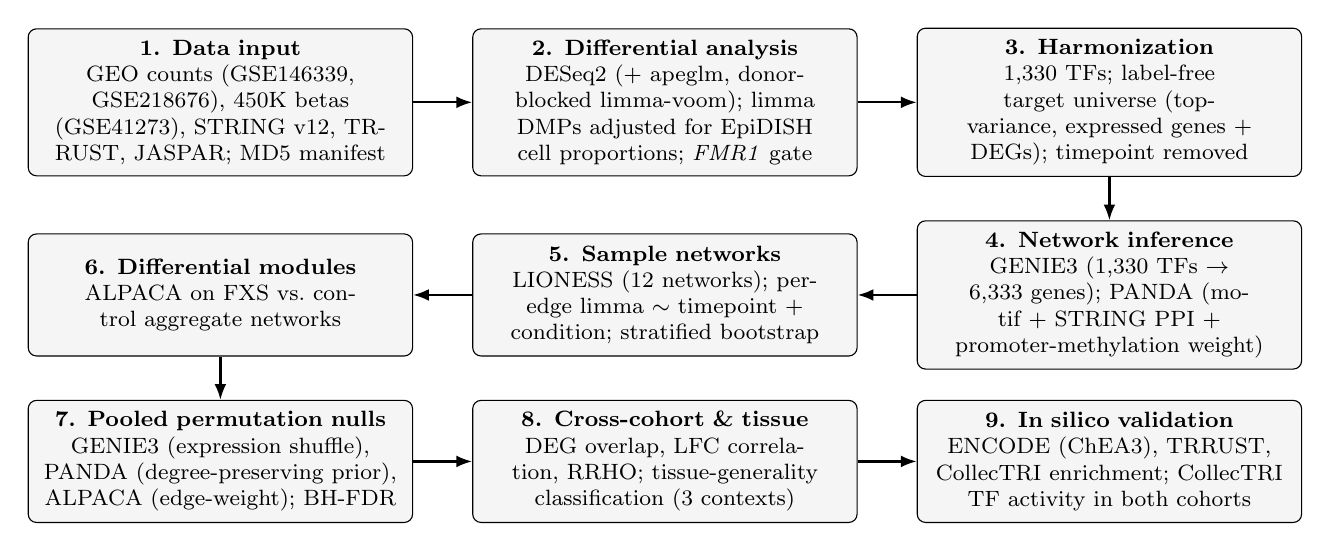
\begin{tikzpicture}[
  box/.style={draw, rounded corners=3pt, fill=gray!8, align=center, font=\footnotesize,
              text width=4.6cm, minimum height=1.55cm, inner sep=4pt},
  arr/.style={-{Latex[length=2mm]}, thick},
  node distance=0.55cm and 0.75cm]
\node[box] (b1) {\textbf{1. Data input}\\ GEO counts (GSE146339, GSE218676), 450K betas (GSE41273), STRING v12, TRRUST, JASPAR; MD5 manifest};
\node[box, right=of b1] (b2) {\textbf{2. Differential analysis}\\ DESeq2 (+ apeglm, donor-blocked limma-voom); limma DMPs adjusted for EpiDISH cell proportions; \gene{FMR1} gate};
\node[box, right=of b2] (b3) {\textbf{3. Harmonization}\\ 1,330 TFs; label-free target universe (top-variance, expressed genes + DEGs); timepoint removed};
\node[box, below=of b3] (b4) {\textbf{4. Network inference}\\ GENIE3 (1,330 TFs $\rightarrow$ 6,333 genes); PANDA (motif + STRING PPI + promoter-methylation weight)};
\node[box, left=of b4] (b5) {\textbf{5. Sample networks}\\ LIONESS (12 networks); per-edge limma $\sim$ timepoint + condition; stratified bootstrap};
\node[box, left=of b5] (b6) {\textbf{6. Differential modules}\\ ALPACA on FXS vs.\ control aggregate networks};
\node[box, below=of b6] (b7) {\textbf{7. Pooled permutation nulls}\\ GENIE3 (expression shuffle), PANDA (degree-preserving prior), ALPACA (edge-weight); BH-FDR};
\node[box, right=of b7] (b8) {\textbf{8. Cross-cohort \& tissue}\\ DEG overlap, LFC correlation, RRHO; tissue-generality classification (3 contexts)};
\node[box, right=of b8] (b9) {\textbf{9. In silico validation}\\ ENCODE (ChEA3), TRRUST, CollecTRI enrichment; CollecTRI TF activity in both cohorts};
\draw[arr] (b1) -- (b2); \draw[arr] (b2) -- (b3); \draw[arr] (b3) -- (b4);
\draw[arr] (b4) -- (b5); \draw[arr] (b5) -- (b6); \draw[arr] (b6) -- (b7);
\draw[arr] (b7) -- (b8); \draw[arr] (b8) -- (b9);
\end{tikzpicture}
\caption{Computational workflow. Each box is one stage; the flow runs left to right and snakes top to bottom. Every network-level statistic (stage 7) is tested against a pooled null before biological interpretation.}
\label{fig:workflow}
\end{figure*}

The two RNA-seq cohorts differ in tissue and cell type, and the methylation cohort adds a third, non-overlapping tissue. We use this as three independent windows onto the same lesion: a gene significant in two or more contexts is more plausibly a tissue-general consequence of \gene{FMR1} loss, and one significant in a single context more plausibly tissue-specific. This framing assumes that discordance reflects biology rather than processing differences, which we mitigate by using NCBI-reprocessed gene-level counts for both RNA-seq cohorts. The methylation cohort has no paired RNA-seq, so it indicates whether epigenetic changes are tissue-general or focal and supplies a population-level prior; it does not support subject-level multi-omic integration.

\section{Methodology}
\subsection{Implementation}
The pipeline is five R scripts run in sequence, each in a fresh R session (\repo{scripts/part1_steps1-8.R} to \repo{scripts/part4_steps20-22.R}, plus \repo{scripts/17b-run.R}), with shared configuration in \repo{scripts/00_config.R}. All analyses reported here were run on Google Colab (2 vCPU, 12.7\,GB RAM) with R~4.6 and Bioconductor~3.23 installed from binary packages; exact package versions and session information for every stage are in \repo{logs/}. Random seeds are fixed throughout, and every permutation loop checkpoints after each iteration.

\subsection{RNA-seq Differential Expression}\label{sec:de}
Counts were analyzed with DESeq2~\cite{deseq2} (Wald test; significance at adjusted $p<0.05$ and $|\log_2\mathrm{FC}|>1$), using $\sim$ timepoint + condition in the primary cohort and $\sim$ cell type + condition in the validation cohort. Gene symbols were mapped from Entrez IDs with \texttt{org.Hs.eg.db}. As a check on sample labels, \gene{FMR1} was required to be significantly downregulated in FXS before proceeding; both cohorts passed. Shrunken effect sizes (apeglm~\cite{apeglm}) were computed alongside unshrunken ones for cross-cohort correlation. Because two validation donors contribute two lines each, we repeated the validation analysis with limma-voom~\cite{voom} treating donor as a blocking factor (\texttt{duplicateCorrelation}~\cite{dupcor}).

\subsection{Differential DNA Methylation}
Beta values for GSE41273 were taken from the GEO series matrix (485,497 probes; values verified to lie in $[0,1]$). Leukocyte proportions (B, NK, CD4$^+$ T, CD8$^+$ T, monocytes, neutrophils, eosinophils) were estimated with EpiDISH~\cite{epidish} (robust partial correlation, blood reference) and included as covariates, omitting neutrophils because proportions sum to one. DMPs were called with limma~\cite{limma} at adjusted $p<0.05$ and $|\Delta\beta|>0.1$; the unadjusted model ($\sim$ condition) is reported as a sensitivity analysis. Probes were annotated with the IlluminaHumanMethylation450k annotation via minfi~\cite{minfi}, expanded to all annotated genes, and summarized as gene-level mean $\Delta\beta$.

\subsection{TF List, Timepoint Adjustment and Target Universe}\label{sec:universe}
A curated list of 1,390 human TFs (\repo{data/tf_list.txt}) was intersected with the expression matrix, retaining 1,330 TFs. In the primary cohort, developmental timepoint dominates the first principal component ($|r|=0.96$ with PC1); because co-expression driven by timepoint would otherwise be read as regulation, timepoint was regressed out of the variance-stabilized expression matrix used for all network inference (limma \texttt{removeBatchEffect}, protecting the condition effect), reducing $|r|$ to 0. Differential expression was unaffected, since DESeq2 models timepoint directly.

Candidate targets were chosen without using FXS/control labels: non-TF genes with at least 10 normalized counts in at least 3 samples (18,107 of 22,011), ranked by variance, of which the top 5,000 were kept, together with all DEGs. The GENIE3 universe therefore comprised 6,333 genes (1,330 TFs, 5,003 non-TF targets; 22.1\% of the 28,679-gene matrix). PANDA's motif target pool was drawn from the same ranked list (3,000 non-TF genes), so neither network's gene selection depends on the contrast later tested. Six TFs previously reported in the FXS literature---SP1, NRF1, REST, FOXG1, SIX3 and TFAP2A---were fixed a priori as reference regulators and used only to examine the recovered networks.

\subsection{GENIE3}
GENIE3~\cite{genie3} was run with the 1,330 TFs as candidate regulators of all 6,333 genes (1,000 trees per target). Its weight matrix is indexed regulator $\times$ target and normalized per target; we verified both properties in the output (per-target weight sums equal to 1). Edges with zero weight and self-edges were discarded, leaving 8,260,380 TF$\rightarrow$gene edges. Hub TFs were ranked by weighted out-degree.

\subsection{PANDA}
A motif prior was built by scanning hg38 promoters ($-2{,}000$ to $+500$\,bp) of the 2,802 target genes with annotated promoters against JASPAR~2020~\cite{jaspar2020} motifs (523 TFs with motifs; 373,665 motif edges). The PPI prior used high-confidence STRING v12.0~\cite{string2023} interactions (combined score $\geq700$; 473,860 edges); STRING protein identifiers were mapped to gene symbols with STRING's own protein-information table, which mapped all 16,201 proteins and yielded 6,490 TF--TF interactions. Motif-prior edges were reweighted by a continuous function of control-group promoter methylation, $1.5-\beta_{\text{promoter}}$ (74.9\% of targets had promoter probes; the remainder received the median), so that the prior encodes baseline promoter accessibility rather than the FXS contrast; this modulated 93.7\% of motif edges (Fig.~\ref{fig:methweight}). PANDA~\cite{panda} (union mode) converged on 873 TFs and 3,325 genes.

\begin{figure}[!t]
\centering
\twofig{methylation_weighting_effect.png}{promoter_methylation_distribution.png}
\caption{Methylation-derived accessibility prior. Left: PANDA motif scores before vs.\ after reweighting by $1.5-\beta_{\text{promoter}}$; points below the diagonal are down-weighted by promoter methylation. Right: distribution of control-group promoter methylation used to derive the weight.}
\label{fig:methweight}
\end{figure}

\subsection{Sample-Specific Networks: LIONESS}
LIONESS~\cite{lioness} in PANDA mode produced one network per primary-cohort sample (12 networks, 2,902,725 edges each). Differential edges were tested by fitting each edge's 12 sample-specific weights with limma, $\sim$ timepoint + condition, with Benjamini--Hochberg (BH) correction. As a genome-wide summary, we computed the proportion of edges stronger in the FXS mean than in the control mean, with a 95\% bootstrap interval (1,000 resamples, stratified by timepoint within each group).

\subsection{Differential Modularity: ALPACA}
FXS and control aggregate networks were the means of the corresponding LIONESS networks. ALPACA~\cite{alpaca} detected communities in the control network and scored each node's contribution to differential modularity in FXS.

\subsection{Pooled Permutation Nulls}\label{sec:nulls}
Each network statistic was compared with a null distribution generated by repeating the inference step under a null model: for GENIE3, each gene's expression vector was shuffled independently (destroying co-expression while preserving marginals; GENIE3 does not use labels, so label permutation would be uninformative); for PANDA, the motif prior was rewired with degree preservation and its scores shuffled; for ALPACA, FXS edge weights were permuted over the fixed network topology. We used 20 permutations for each (250 trees per target for the GENIE3 null, which widens the null and makes the test conservative).

A per-edge null---comparing each edge only with its own permutation values---cannot support FDR control at this scale: with $B$ permutations the smallest attainable $p$ is $1/(B+1)$ (0.048 for $B=20$), whereas BH correction over $\sim$$10^6$--$10^7$ edges requires $p$-values several orders of magnitude smaller, so ``zero edges at FDR $<0.05$'' would be guaranteed regardless of the data. We therefore compared each observed score $x$ with the pooled null of all edges (or nodes) across all permutations, $p=(\#\{\text{null}\geq x\}+1)/(N+1)$, accumulated in a constant-memory histogram (200,000 bins; a bin straddling $x$ is counted as exceeding it, so $p$ is conservative). This assumes scores are comparable across edges, which holds for GENIE3 (weights normalized per target over a common regulator set) and PANDA ($z$-scaled scores). Smallest attainable $p$ was $8.6\times10^{-9}$ (GENIE3) and $1.7\times10^{-8}$ (PANDA). ALPACA module significance compared each module's mean node score with $10^5$ random draws of the same size from the pooled node null; stability was checked by repeating the test with the first 10 permutations only. All $p$-values were BH-corrected.

\subsection{Tissue-Generality Classification}\label{sec:tissue}
Each gene significant in at least one tissue context (primary DEG, validation DEG, or DMP-annotated gene) was called tissue-general if significant in at least two of the three contexts and tissue-specific if significant in exactly one. Methylation gene names from the hg19-era 450K annotation were mapped to current symbols (e.g.\ \gene{ASFMR1} $\rightarrow$ \gene{FMR1-AS1}), and probes in the shared \gene{FMR1}/\gene{FMR1-AS1} promoter count towards both. Genes significant in no context were excluded. For each pair of contexts, the overlap was compared with its hypergeometric expectation on the shared gene background. Because contexts differ in sample size and modality, the classification is descriptive.

\subsection{Functional Enrichment}
GO Biological Process and KEGG enrichment were run with clusterProfiler~\cite{clusterprofiler} for each ALPACA module (at least 5 genes) and for the top-scoring ALPACA genes, against the network gene universe, at strict (BH-adjusted $p<0.05$) and relaxed (BH-adjusted $p<0.1$) thresholds.

\subsection{Cross-Cohort Validation}
The primary and validation cohorts were compared on the 26,014 genes testable in both: (i) DEG overlap (hypergeometric and Fisher's exact tests); (ii) genome-wide effect-size correlation (Pearson, Spearman) and sign concordance, on raw and apeglm-shrunken log$_2$FC; and (iii) rank--rank hypergeometric overlap (RRHO)~\cite{rrho} of genes ranked by signed $-\log_{10}p$, on a $99\times99$ grid of rank cutoffs using our implementation of the original algorithm.

\subsection{In Silico Regulator Validation}
For candidate TFs (top hubs plus the reference TFs with database coverage), the top 200 (ENCODE) or 500 (TRRUST, CollecTRI) predicted targets from each network were tested against three independent sources: self-recovery rank among ENCODE ChIP-seq regulator libraries~\cite{encode2012} returned by ChEA3~\cite{chea3}; and hypergeometric enrichment among curated targets in TRRUST~v2~\cite{trrust} and CollecTRI~\cite{collectri} (43,159 interactions, 1,186 TFs; retrieved 9~November~2026), with BH correction. Separately, TF activity was inferred in each cohort from the DESeq2 Wald statistics and CollecTRI regulons with a univariate linear model (decoupleR~\cite{decoupler}; minimum regulon size 5), giving a TF-level cross-cohort comparison that does not require individual target genes to replicate.

\section{Results}
\subsection{Differential Expression and Methylation}
DESeq2 identified 13 DEGs in the primary organoid cohort (12 down, 1 up), led by \gene{FMR1} (log$_2$FC $=-10.47$, $p_{\text{adj}}=3.1\times10^{-51}$) and \gene{FMR1-AS1} ($-5.08$, $p_{\text{adj}}=2.7\times10^{-3}$); the remainder include Hedgehog and patterning genes (\gene{SHH}, \gene{GLI1}, \gene{PITX2}, \gene{HOXA2}, \gene{HOTAIRM1}; Figs.~\ref{fig:de},~\ref{fig:heatmap}). In the validation cohort, 63 genes were significant with lines treated as independent, and \gene{FMR1} replicated (log$_2$FC $=-8.91$, $p_{\text{adj}}=7.2\times10^{-8}$). The donor-blocked analysis, however, estimated a within-donor correlation of 0.66 and retained only one significant gene, \gene{FMR1} (log$_2$FC $=-9.19$, FDR $=0.031$), although effect sizes agreed closely between the two models (Pearson $r=0.84$). The 63 validation DEGs should therefore be read as nominal at the line level; \gene{FMR1} is the only validation DEG robust to donor structure.

\begin{figure}[!t]
\centering
\twofig{PCA_GSE146339.png}{volcano_plot_FXS_vs_Control.png}
\caption{Differential expression, GSE146339. Left: PCA (PC1 separates day 28 from day 105). Right: volcano plot, FXS vs.\ Control.}
\label{fig:de}
\end{figure}

\begin{figure}[!t]
\centering
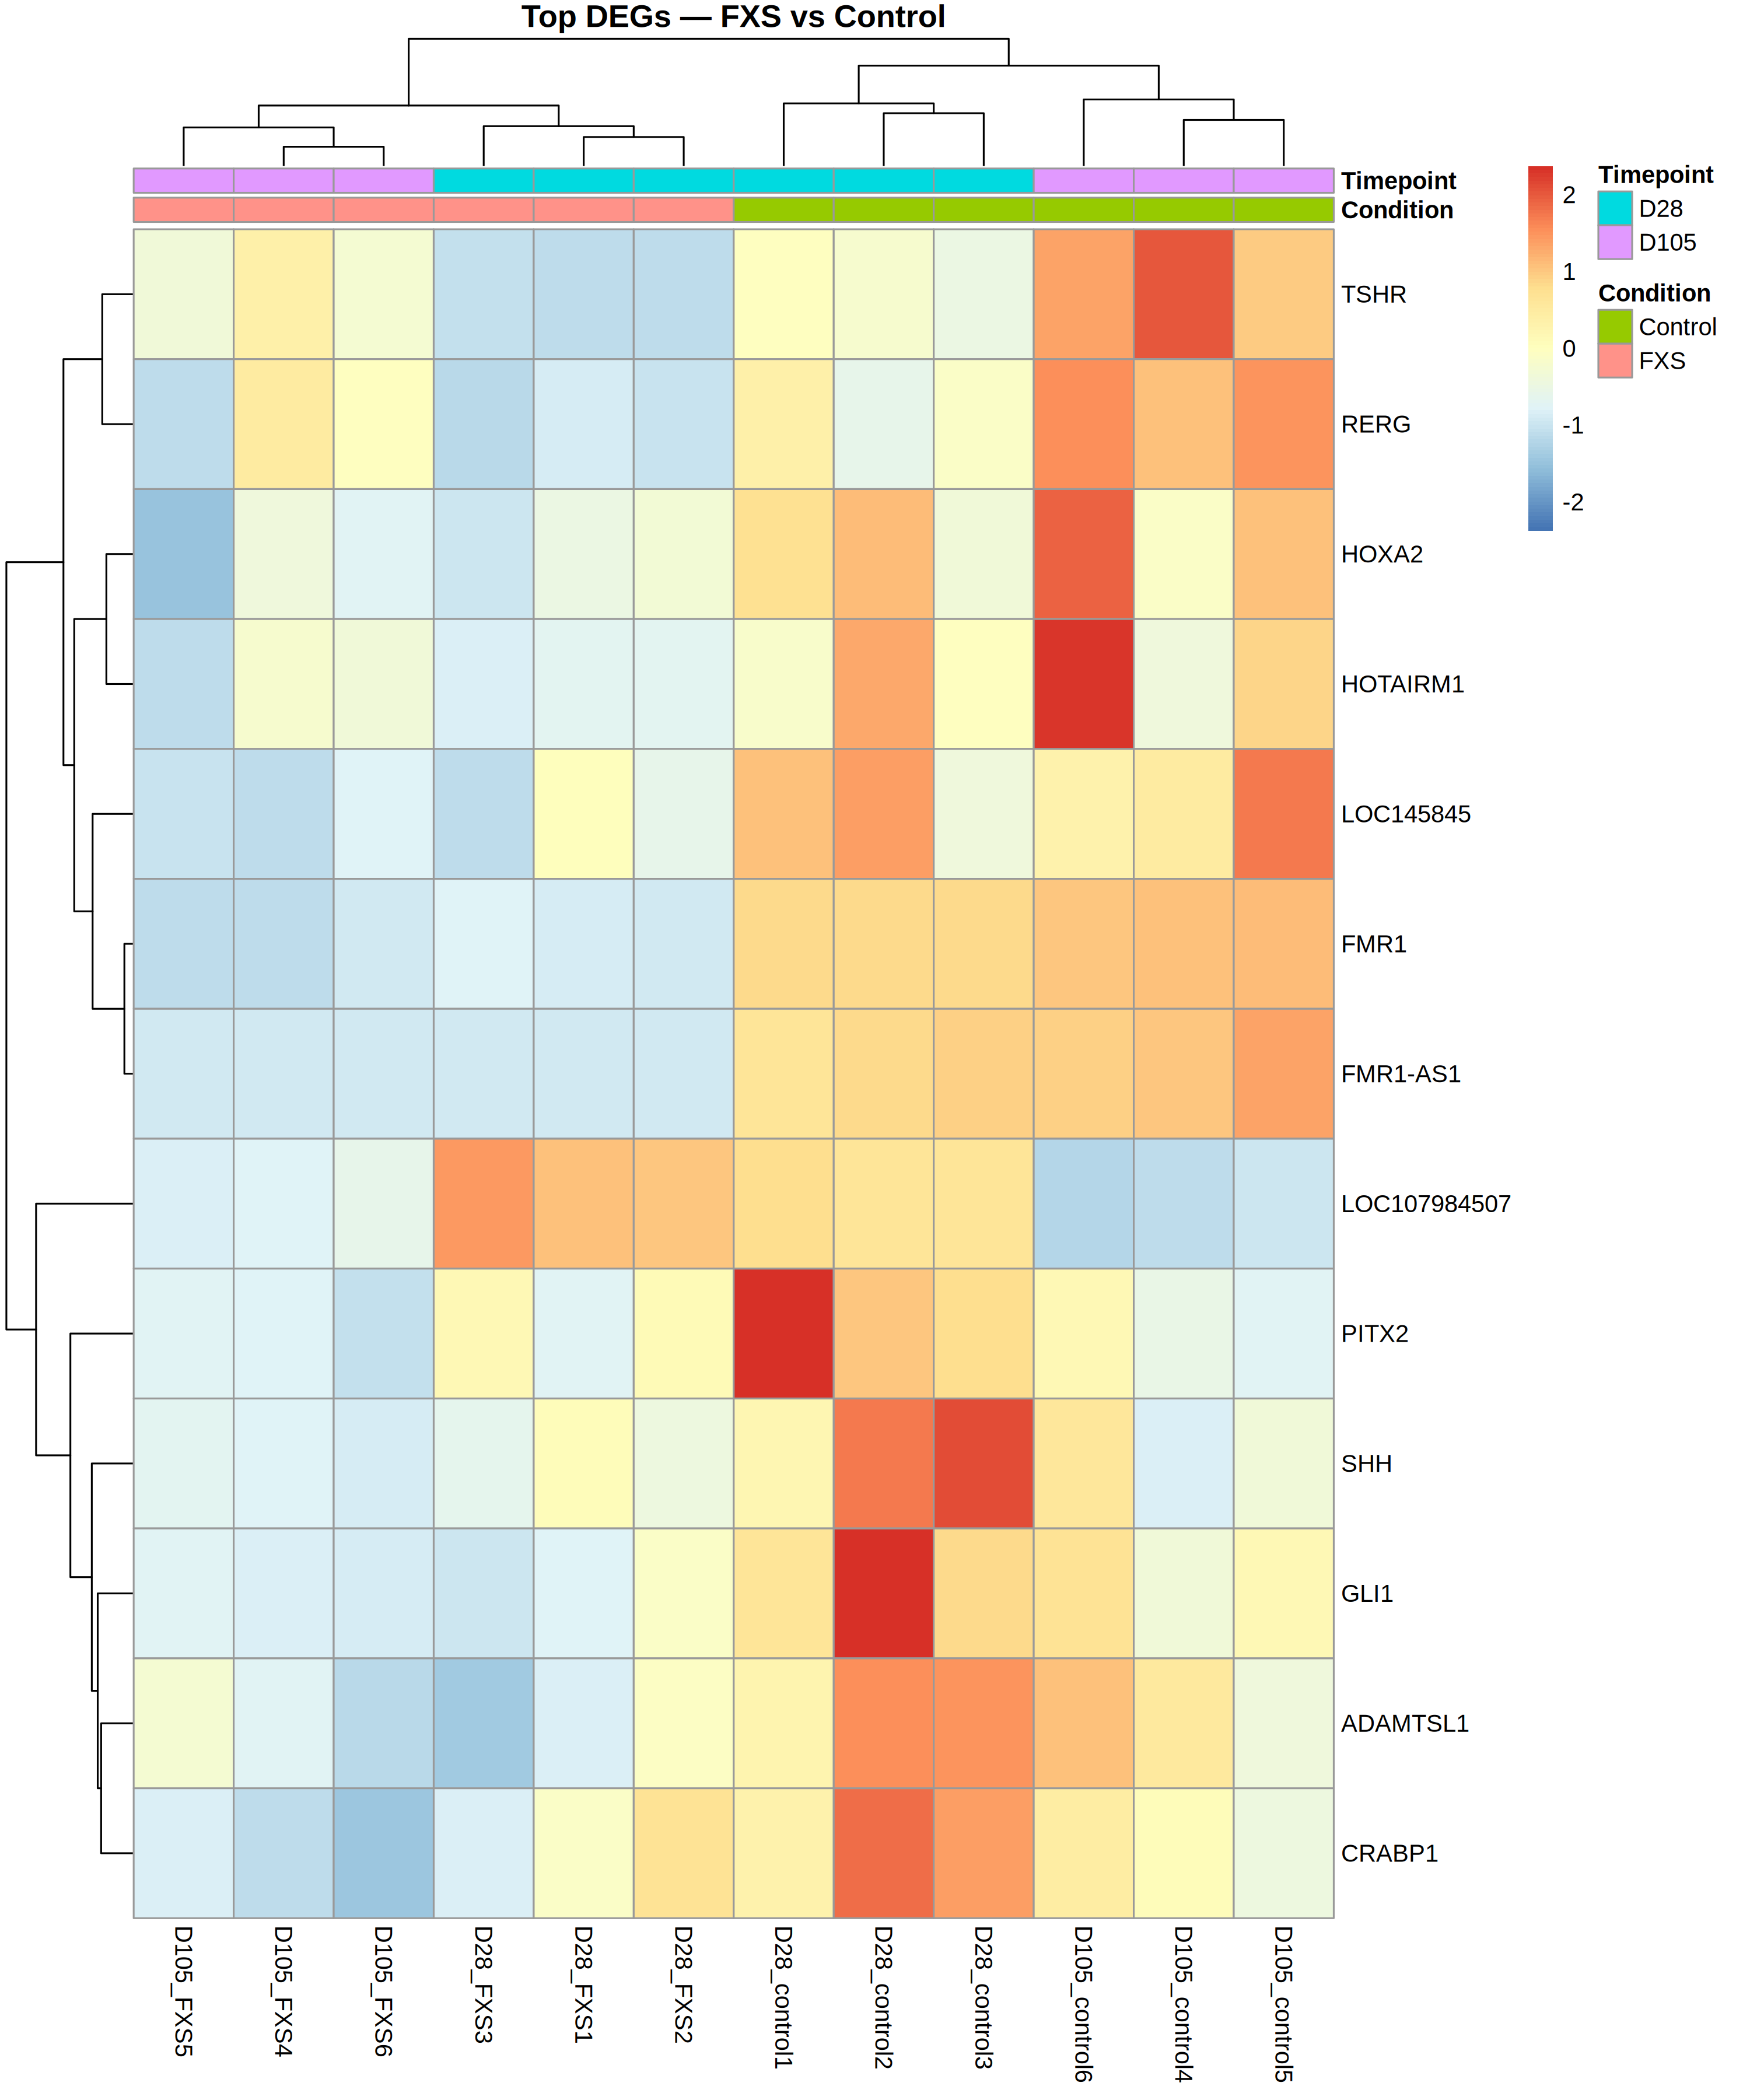
\includegraphics[width=\columnwidth]{heatmap_top_DEGs.png}
\caption{The 13 differentially expressed genes, GSE146339, led by \gene{FMR1} and \gene{FMR1-AS1}.}
\label{fig:heatmap}
\end{figure}

In blood, estimated CD8$^+$ T-cell and eosinophil proportions differed between FXS and controls (Wilcoxon $p=0.013$ and $0.002$), confirming that composition adjustment was needed. The adjusted model identified 41 DMPs (FDR $<0.05$, $|\Delta\beta|>0.1$) in 21 genes (9 hyper-, 12 hypomethylated); the unadjusted model reproduced the 25 DMPs of a composition-naive analysis. \gene{FMR1}/\gene{FMR1-AS1} dominated under both models (mean $\Delta\beta=0.582$ adjusted, 0.562 unadjusted, 15 shared promoter probes), while every other DMP gene had $|\Delta\beta|$ between 0.10 and 0.18 (Fig.~\ref{fig:meth}). Hypermethylation is thus strongly focal at the causal locus, as expected; we treat this as an internal validity check rather than a new mechanistic finding.

\begin{figure}[!t]
\centering
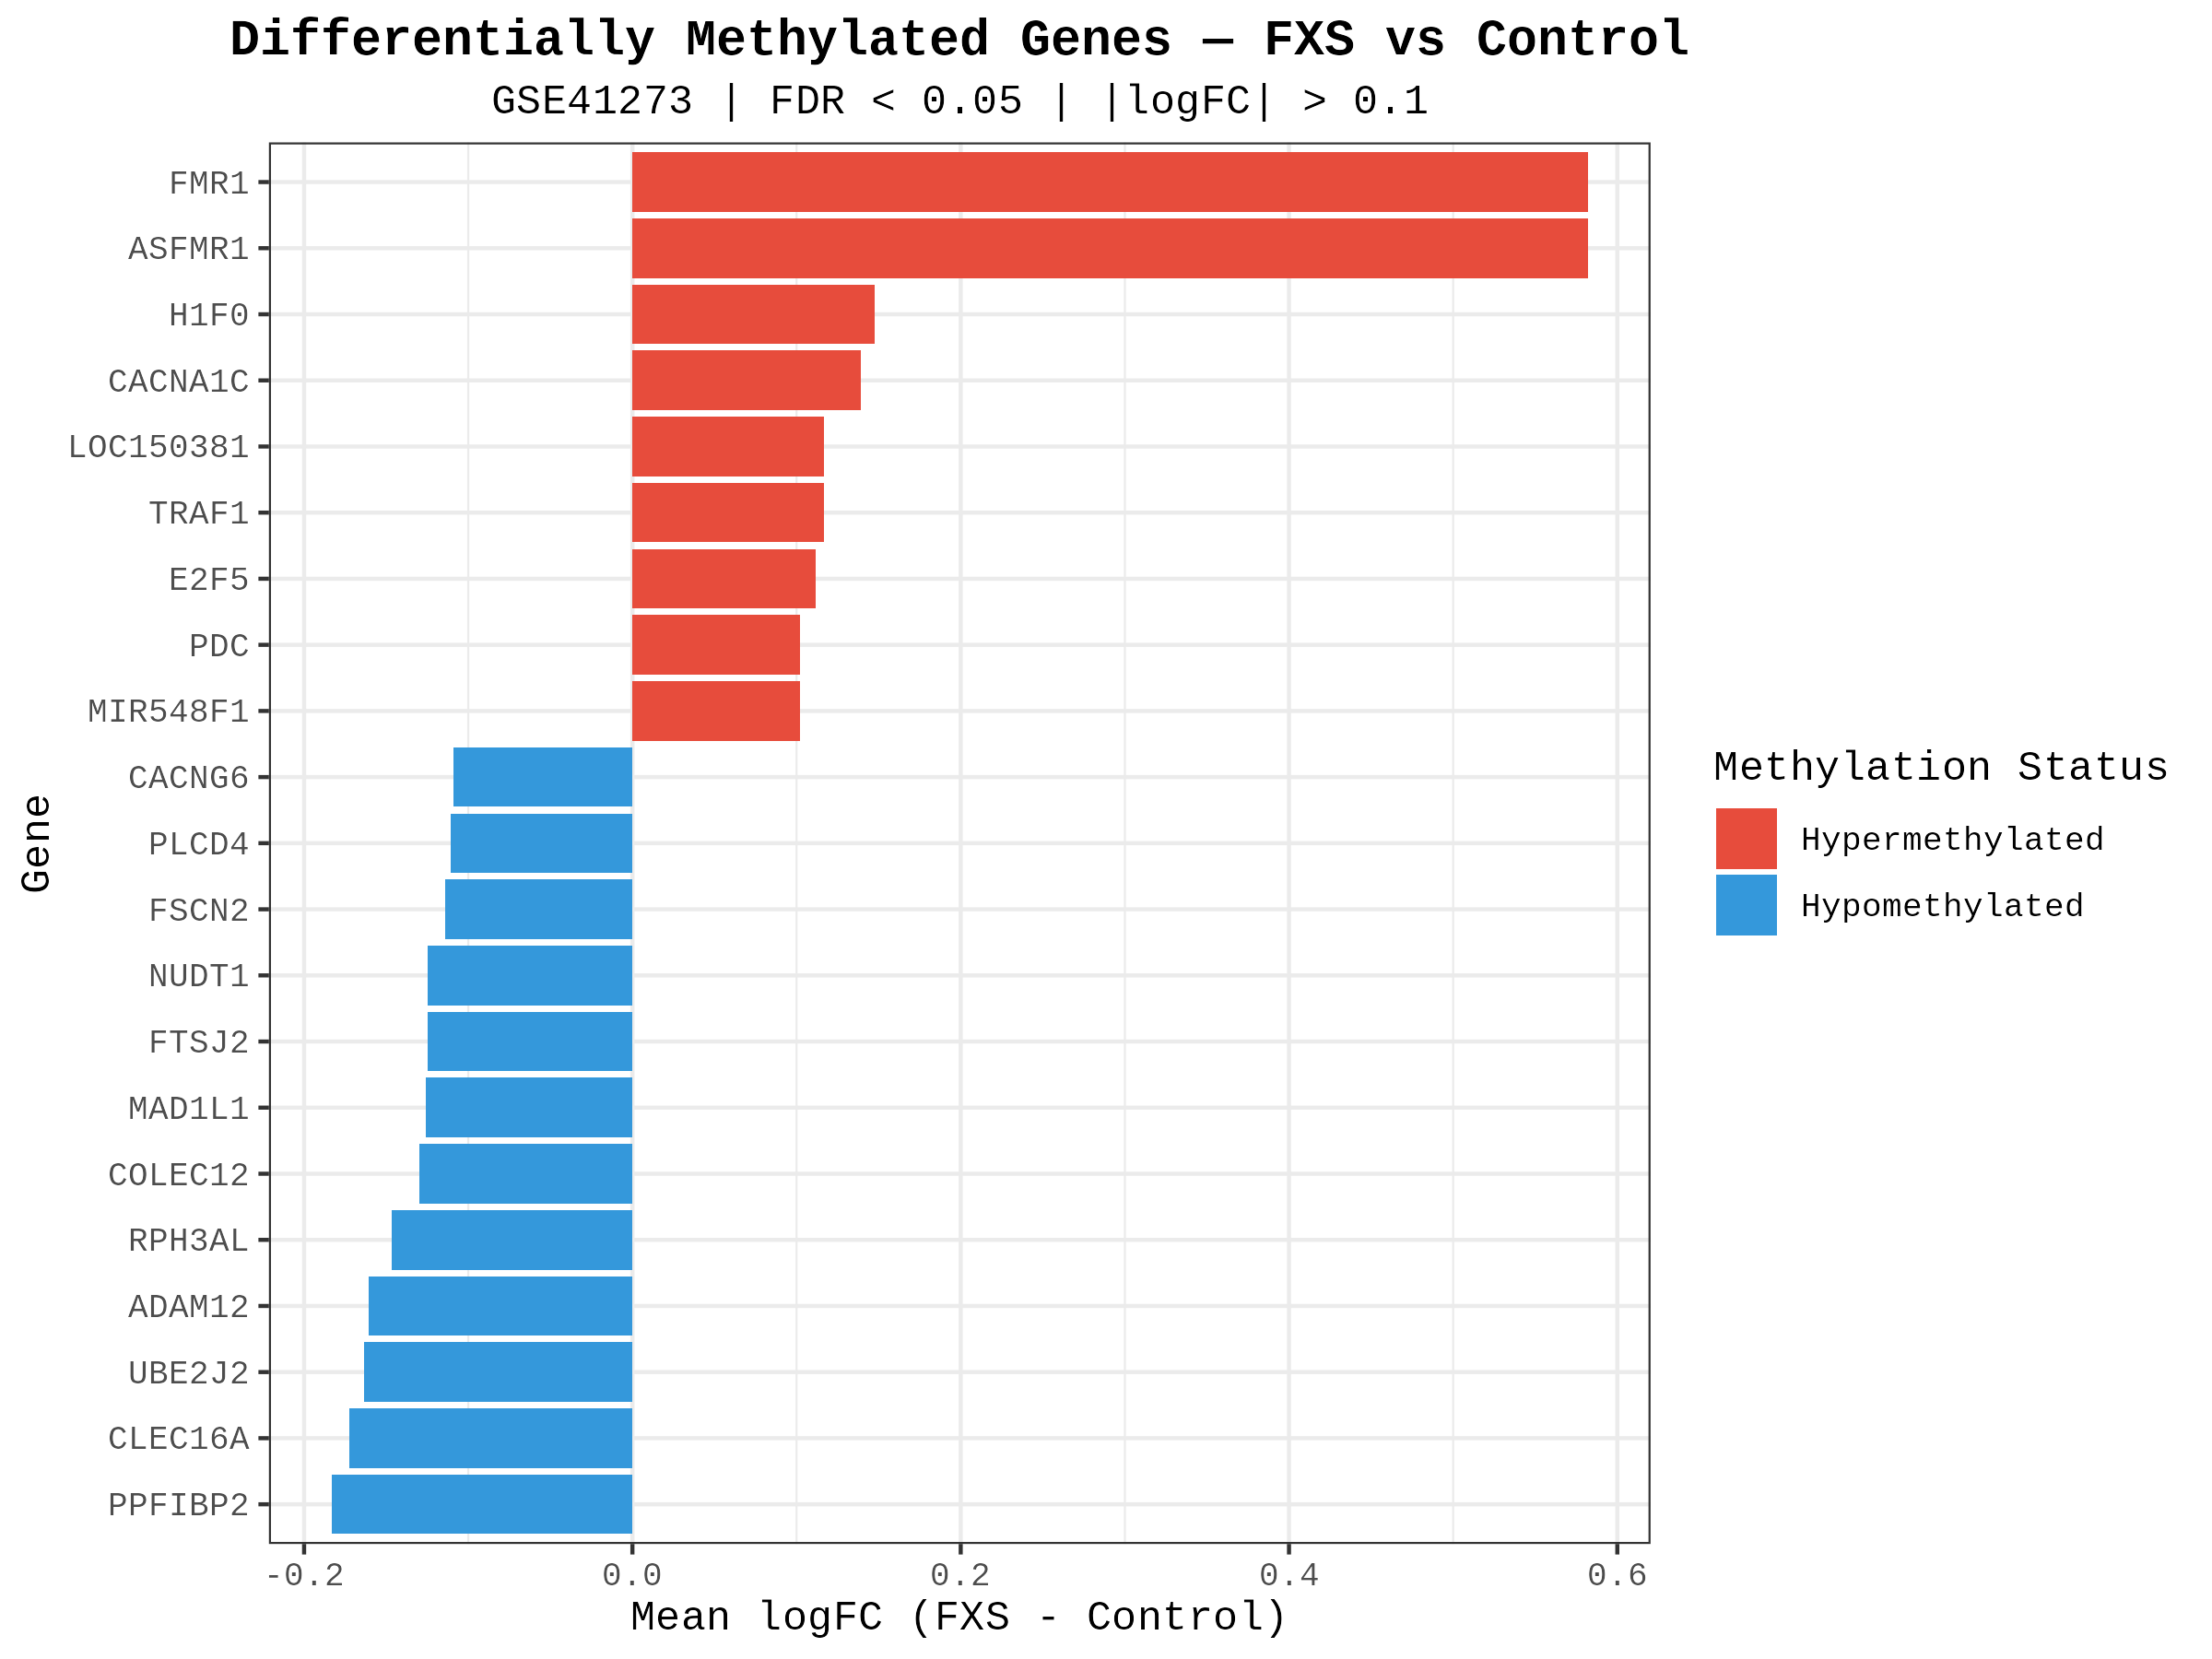
\includegraphics[width=0.92\columnwidth]{methylation_gene_summary.png}
\caption{Differentially methylated genes, GSE41273 (cell-composition-adjusted; FDR $<0.05$, $|\Delta\beta|>0.1$). \gene{FMR1} and \gene{ASFMR1} (\gene{FMR1-AS1}) share 15 promoter probes.}
\label{fig:meth}
\end{figure}

\subsection{GENIE3 and PANDA Networks}
For visualization and hub ranking, we retained the top 1\% of GENIE3 edges (82,604 edges; 6,168 nodes, 1,330 TFs) and the top decile of positive PANDA edges (100,968 edges; 3,245 nodes, 518 TFs; Fig.~\ref{fig:networks}). Top GENIE3 hubs by weighted out-degree were MEIS3, HESX1 and ARID5B; top PANDA hubs were ZNF460, ZNF384, IRF1 and KLF5 (Fig.~\ref{fig:hubs}). Of the six reference TFs, REST ranked 29th of 1,330 TFs in GENIE3 and TFAP2A 48th of 518 in PANDA; the others ranked outside the top 50.

\begin{figure}[!t]
\centering
\twofig{GENIE3_network_plot.png}{PANDA_network_plot.png}
\caption{Inferred TF regulatory networks. Left: GENIE3 (expression only; top 1\% of edges). Right: PANDA (motif + STRING PPI + methylation prior; top decile).}
\label{fig:networks}
\end{figure}

\begin{figure}[!t]
\centering
\twofig{GENIE3_hub_genes.png}{PANDA_hub_genes.png}
\caption{Top 20 hub TFs. Left: GENIE3, weighted out-degree. Right: PANDA, out-degree. Among the reference TFs, REST is in the GENIE3 top 50 and TFAP2A in the PANDA top 50.}
\label{fig:hubs}
\end{figure}

\subsection{Permutation Nulls}
No GENIE3 edge survived FDR $<0.05$: 165,144 of 8,260,380 edges (2.0\%) had pooled $p<0.05$, fewer than the 5\% expected under the null, consistent with the conservative null. For PANDA, 150,070 of 2,902,725 edges (5.2\%) exceeded the null 95th percentile (null $q_{95}=3.55$; observed 90th percentile 3.80), essentially the 5\% expected if the expression data added nothing beyond the priors, and none survived FDR $<0.05$ (Fig.~\ref{fig:null}). Because the PPI prior was fully mapped and the test could reach significance, this indicates that at this sample size PANDA edge scores are driven by prior structure rather than expression.

\begin{figure}[!t]
\centering
\twofig{GENIE3_null_distribution.png}{PANDA_null_distribution.png}
\caption{Pooled permutation nulls. Left: GENIE3 observed edge weights vs.\ expression-shuffled null. Right: PANDA observed edge scores vs.\ degree-preserving randomized-prior null; the distributions nearly coincide.}
\label{fig:null}
\end{figure}

\subsection{Sample-Specific Networks}
In the per-edge LIONESS test adjusted for timepoint, 25,147 of 2,902,725 edges (0.87\%) had nominal $p<0.05$ and none survived FDR $<0.05$. The $p$-value distribution was not uniform but peaked near 0.3 with a deficit near zero (Fig.~\ref{fig:boot}), indicating a conservative test and no excess of small $p$-values. Genome-wide, 52.4\% of edges were stronger in FXS than control (stratified bootstrap 95\% CI 48.3--53.4\%), an interval that includes 50\%: no systematic shift in regulatory strength was detected. Among reference TFs, mean LIONESS edge scores were lower in FXS for NRF1, REST, SP1 and TFAP2A and higher for SIX3 (Fig.~\ref{fig:lion}), descriptive differences that individual edges do not support at FDR.

\begin{figure}[!t]
\centering
\twofig{LIONESS_bootstrap_distribution.png}{LIONESS_limma_pvalue_hist.png}
\caption{LIONESS. Left: stratified bootstrap distribution of the proportion of edges stronger in FXS (95\% CI includes 50\%). Right: per-edge limma $p$-values for the condition effect ($\sim$ timepoint + condition).}
\label{fig:boot}
\end{figure}

\begin{figure}[!t]
\centering
\twofig{LIONESS_top_edges_barplot.png}{LIONESS_known_TF_activity.png}
\caption{LIONESS detail. Left: edges with the largest FXS-vs-control weight differences. Right: mean differential edge score of the six reference TFs across all targets.}
\label{fig:lion}
\end{figure}

\subsection{ALPACA Differential Modules}
ALPACA assigned 3,995 nodes to 249 communities, dominated by three large modules (1,768, 1,557 and 363 nodes); 8 modules had at least 5 nodes. No individual node survived node-level FDR (smallest FDR 0.66). At the module level, one module was significant after correction: module 4 (empirical $p=4\times10^{-5}$, FDR $=0.0099$), which remained significant when the null was built from only the first 10 permutations (FDR $=0.030$). Module 4 has five nodes, including the five highest-scoring nodes in the network: the TFs BARHL1 and OTX1 and the targets \gene{NEFL}, \gene{MPZL2} and \gene{TAF4B}, linked by BARHL1$\rightarrow$\gene{TAF4B}, BARHL1$\rightarrow$\gene{MPZL2} and OTX1$\rightarrow$\gene{NEFL} (Figs.~\ref{fig:alpaca},~\ref{fig:mod4}). BARHL1 and OTX1 are homeobox TFs of neuronal specification and forebrain/midbrain patterning, and \gene{NEFL} encodes the neurofilament light chain; GO terms for this module (BH $p=0.044$) concerned axonal mitochondrial transport and postsynaptic cytoskeleton organization, driven by \gene{NEFL}. Given its size, we regard module 4 as a specific, testable hypothesis rather than an established pathway.

\begin{figure}[!t]
\centering
\twofig{ALPACA_module_significance.png}{ALPACA_top_nodes.png}
\caption{ALPACA. Left: module significance against the pooled null; only module 4 passes (FDR $=0.0099$). Right: top 20 nodes by differential-modularity score, led by the five module-4 nodes.}
\label{fig:alpaca}
\end{figure}

\begin{figure}[!t]
\centering
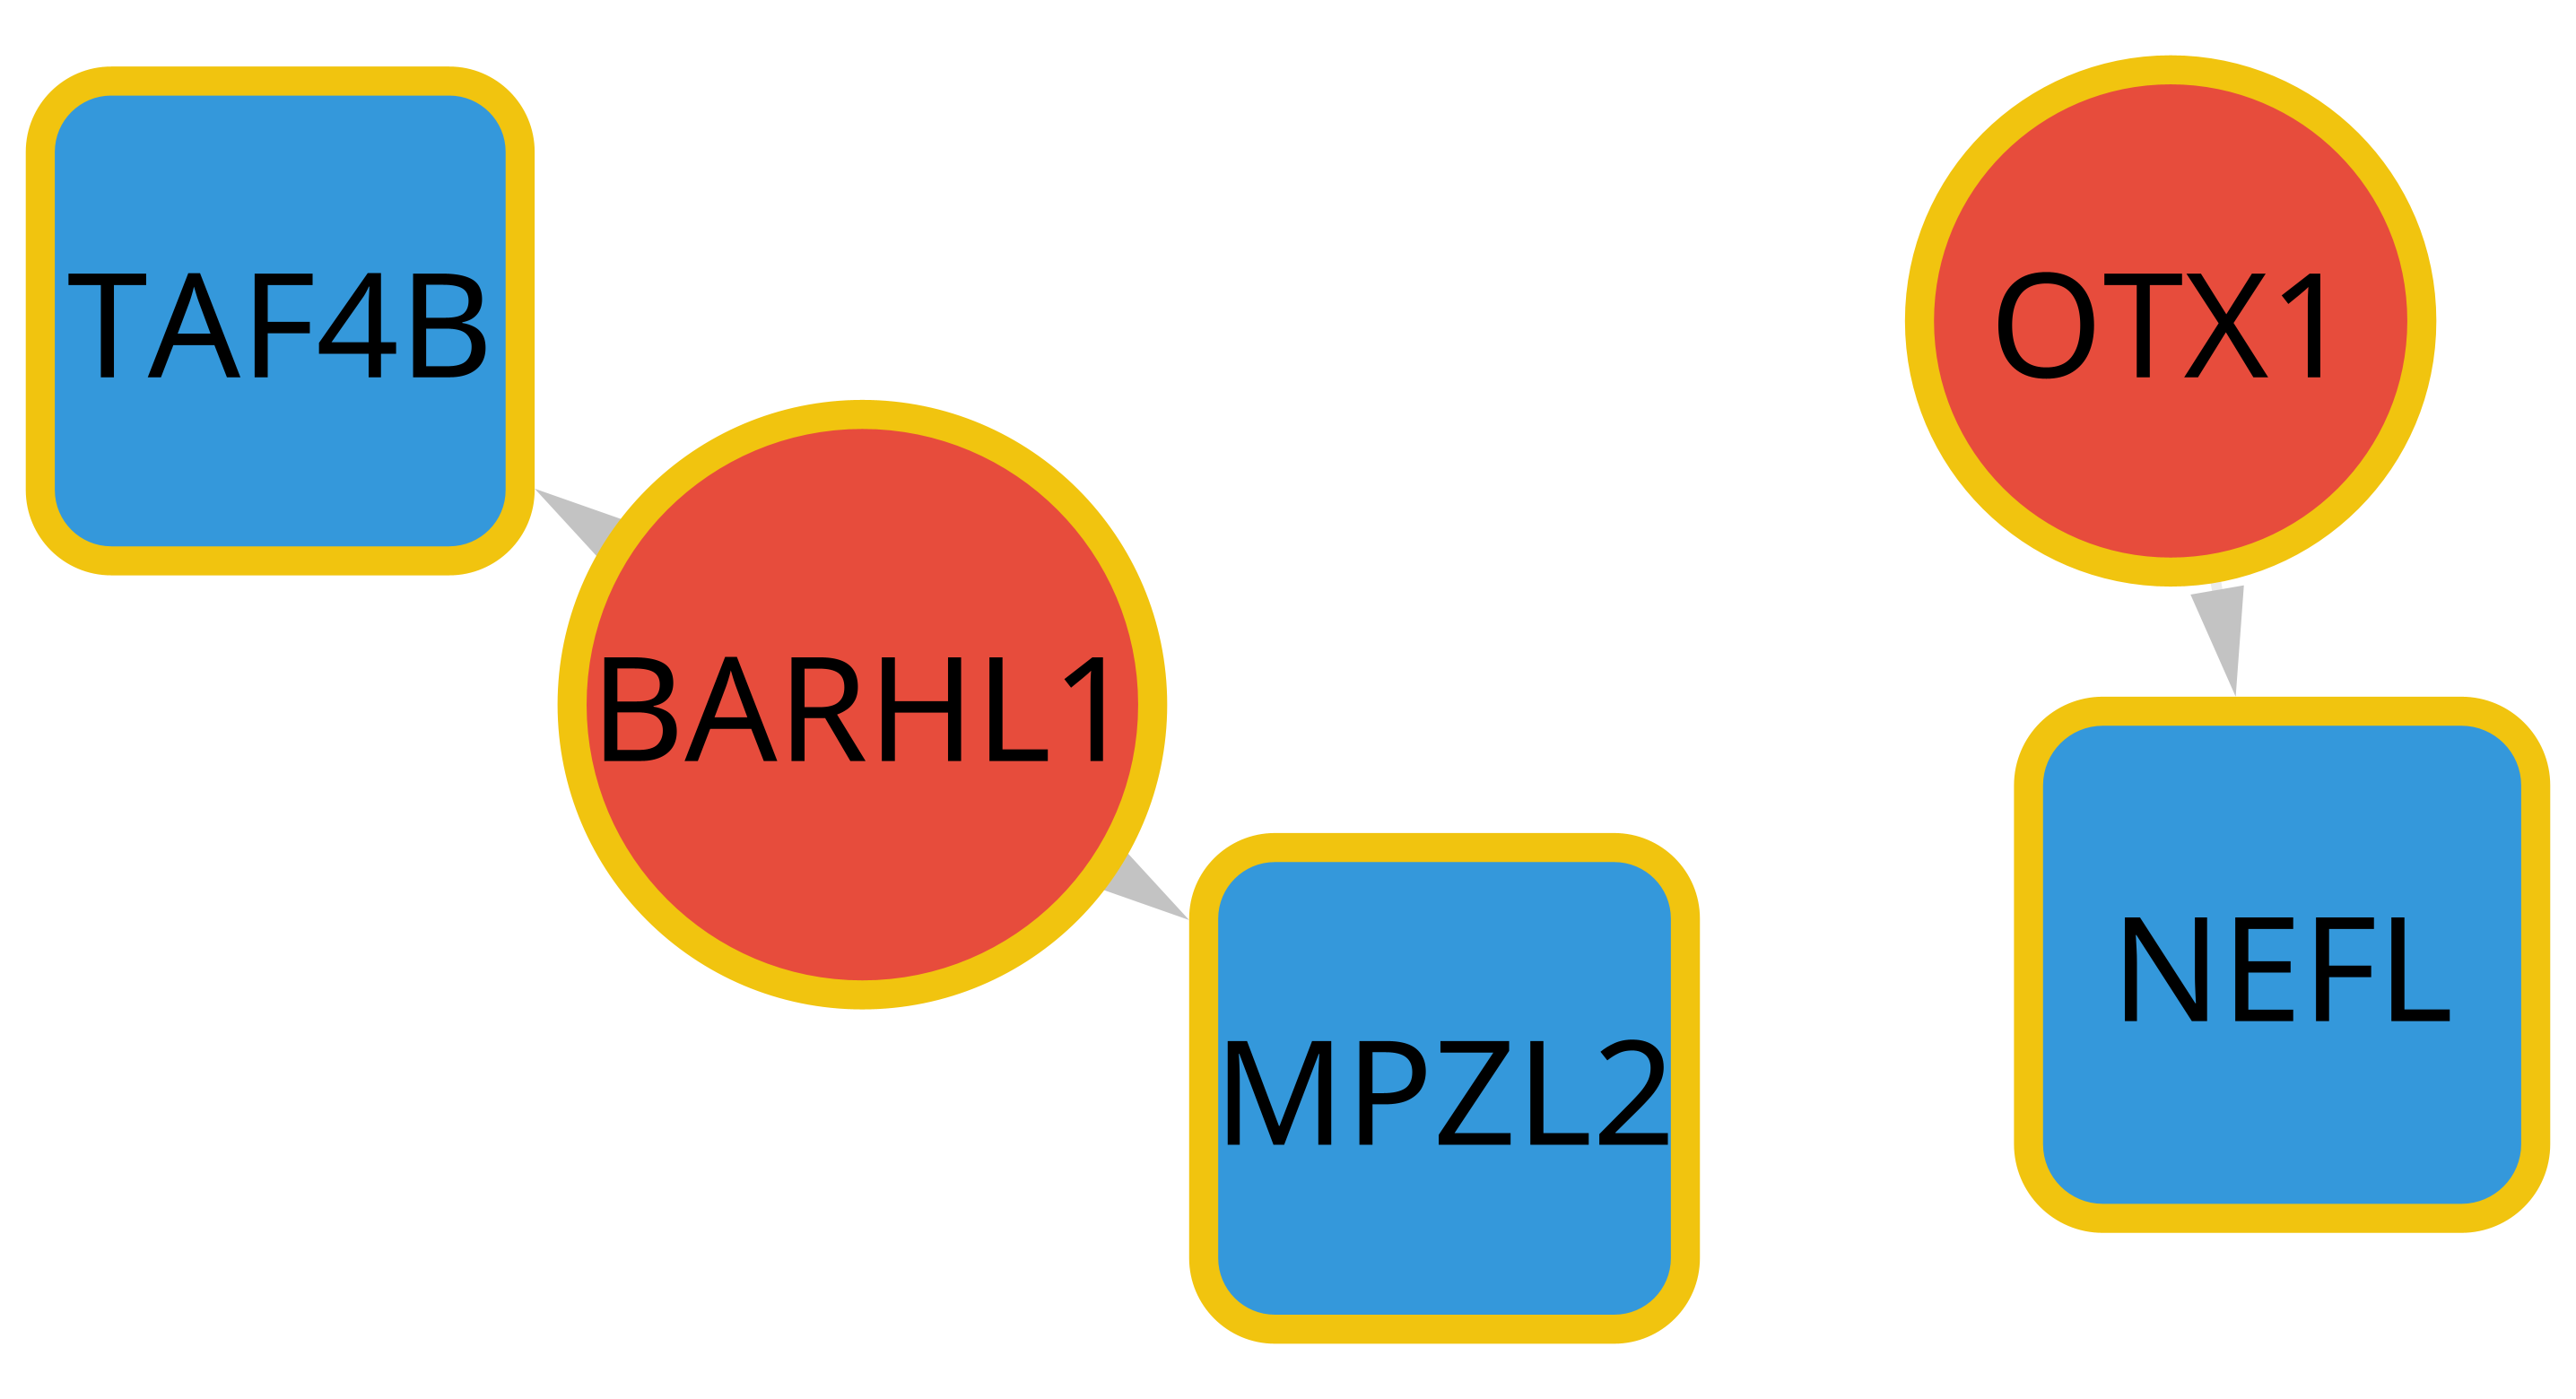
\includegraphics[width=0.8\columnwidth]{FXS_ALPACA_module_4.png}
\caption{ALPACA module 4 (FDR $=0.0099$), drawn in Cytoscape~\cite{cytoscape} via RCy3~\cite{rcy3}. Red circles: TFs; blue squares: targets; arrows: PANDA edges.}
\label{fig:mod4}
\end{figure}

The large modules were enriched for developmental programs: pattern specification and regionalization (module 2, BH $p=1.6\times10^{-21}$), extracellular-matrix organization and response to retinoic acid (module 3), and embryonic morphogenesis (module 1; Fig.~\ref{fig:go}). These modules were not differential against the null, so their enrichments describe network organization rather than FXS effects. The 12 top-scoring ALPACA genes gave no strict GO or KEGG terms; at the relaxed threshold, response to peptide hormone and transcription initiation by RNA polymerase~II (GO), and IL-17 signaling (KEGG) appeared.

\begin{figure}[!t]
\centering
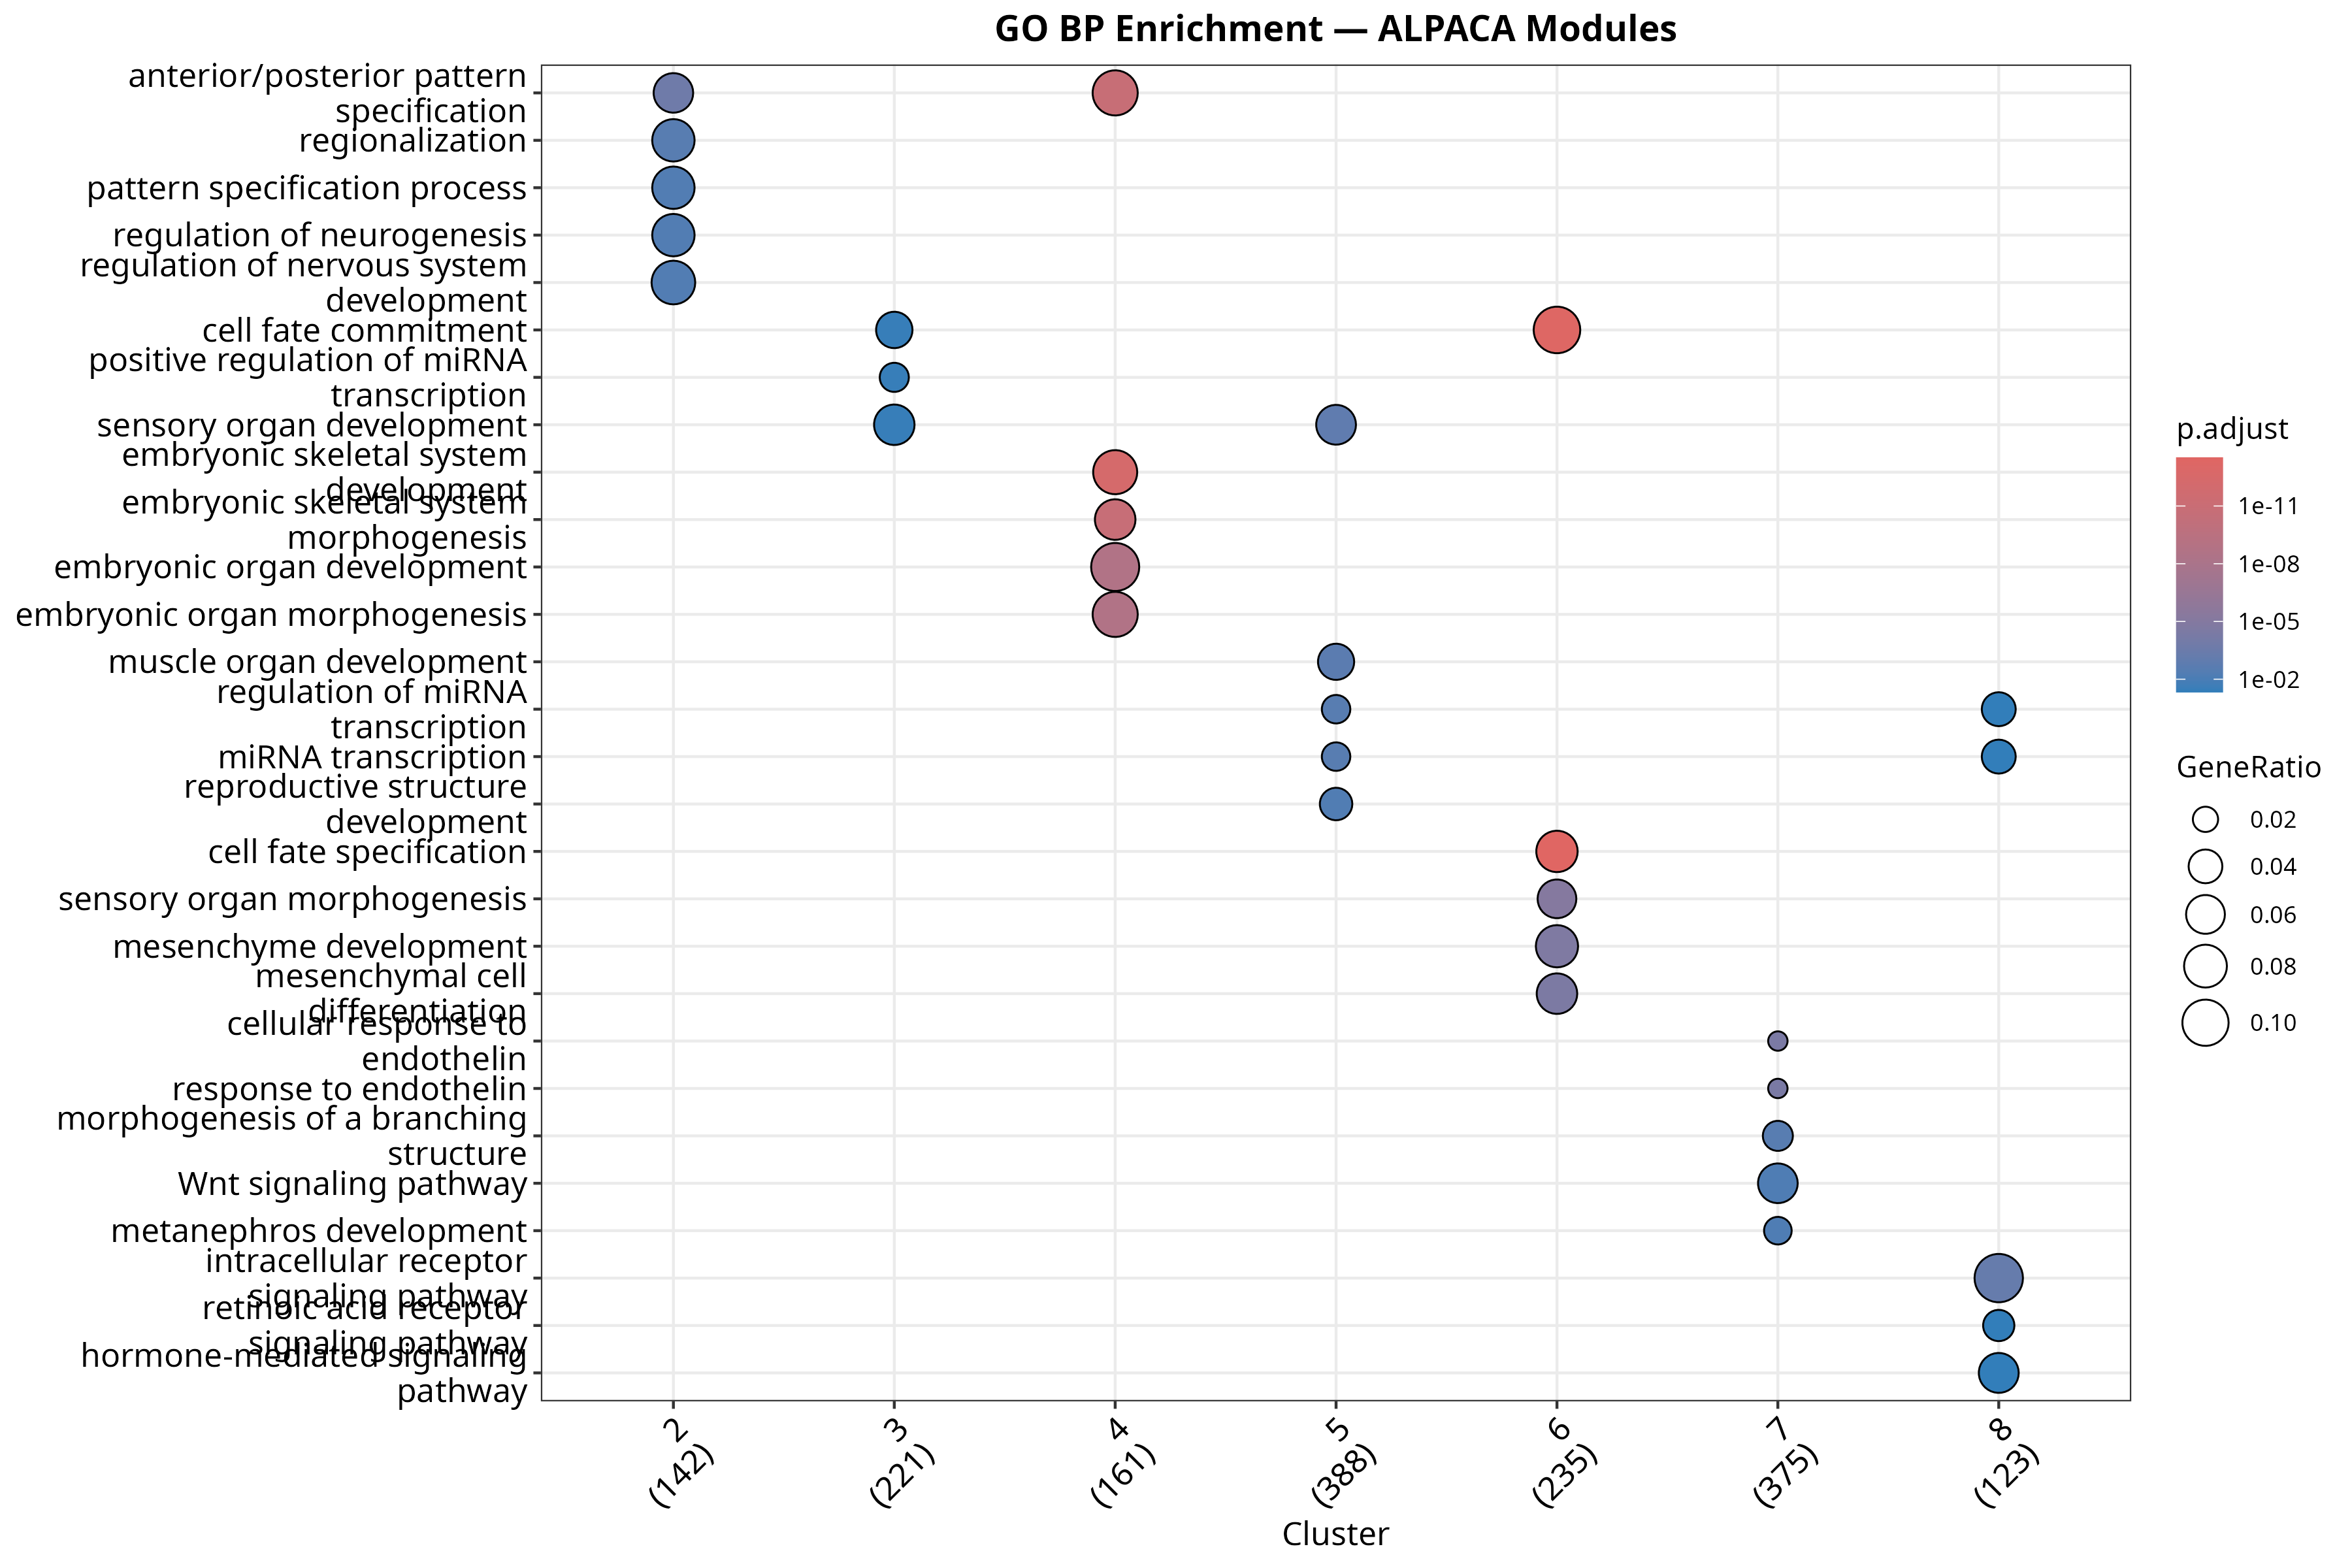
\includegraphics[width=\columnwidth]{ALPACA_module_GO_dotplot.png}
\caption{GO Biological Process enrichment of ALPACA modules with at least 5 genes (BH $p<0.05$). Module 4 terms are driven by \gene{NEFL}.}
\label{fig:go}
\end{figure}

The reference TFs were locally central within their modules despite not being genome-wide hubs: SP1, TFAP2A, NRF1 and REST ranked at the 98th, 98th, 96th and 94th percentiles of within-module weighted strength in module 3, and FOXG1 at the 96th percentile in module 2; SIX3 did not (17th percentile, module 1; Fig.~\ref{fig:local}). Modules 2 and 3 themselves were not differential (FDR $=1$), so this indicates local structural prominence, not FXS-specific rewiring.

\begin{figure}[!t]
\centering
\twofig{FXS_TF_OutDegree_comparison.png}{known_TF_module_local_centrality.png}
\caption{Reference TFs: genome-wide vs.\ module-local relevance. Left: out-degree in GENIE3 and PANDA. Right: percentile of within-module weighted strength (dashed line: top decile).}
\label{fig:local}
\end{figure}

\subsection{Cross-Cohort Validation}
Genome-wide effect sizes barely correlated between cohorts (Pearson $r=0.031$, $p=5.1\times10^{-7}$; Spearman $\rho=0.020$), and sign concordance was 50.5\%, indistinguishable from chance (Fig.~\ref{fig:conc}). Shrinkage did not change this ($r=0.008$, $p=0.19$, shrunken log$_2$FC), so the weak agreement is not an artefact of noisy low-count estimates. RRHO nevertheless detected a concordant region ($-\log_{10}p=13.53$), located at large rank cutoffs in the body of the ranked lists rather than among top-ranked genes (Fig.~\ref{fig:venn}). Only \gene{FMR1} was shared between the primary (13) and validation DEG sets (21 of the 63 testable in both cohorts), concordantly downregulated; given the small set sizes this single-gene overlap is $95\times$ the chance expectation (hypergeometric $p=0.010$; Fisher OR $=108$).

\begin{figure}[!t]
\centering
\twofig{crossvalidation_global_LFC_correlation.png}{crossvalidation_direction_concordance.png}
\caption{Cross-cohort concordance. Left: genome-wide effect sizes across 26,014 shared genes ($r=0.031$; sign concordance 50.5\%). Right: direction of change for the shared DEG, \gene{FMR1} (concordant, 1/1).}
\label{fig:conc}
\end{figure}

\begin{figure}[!t]
\centering
\twofig{crossvalidation_venn.png}{RRHO_manual_heatmap.png}
\caption{Left: DEG overlap between cohorts (only \gene{FMR1}). Right: RRHO heatmap (26,014 genes ranked by signed $-\log_{10}p$; $99\times99$ grid; peak $-\log_{10}p=13.53$).}
\label{fig:venn}
\end{figure}

\subsection{Tissue-General versus Tissue-Specific Effects}
Only \gene{FMR1} and \gene{FMR1-AS1} were tissue-general under the $\geq$2-of-3 rule; \gene{FMR1} was significant in all three contexts, and \gene{FMR1-AS1} in the organoid cohort and the methylation cohort through the shared promoter probes. Of 90 genes significant in exactly one context, 11 were specific to the organoid cohort, 60 to the validation lines and 19 to blood methylation (Fig.~\ref{fig:tissue}). Each pairwise overlap exceeded chance (organoid--blood: 2 genes vs.\ 0.009 expected, $p=3.8\times10^{-5}$), but was carried entirely by the \gene{FMR1} locus. The classification was unchanged when validation DEGs came from the donor-blocked model. Together with the near-zero genome-wide correlation, this indicates that detectable downstream change is almost entirely tissue-restricted, with the causal locus as the exception.

\begin{figure}[!t]
\centering
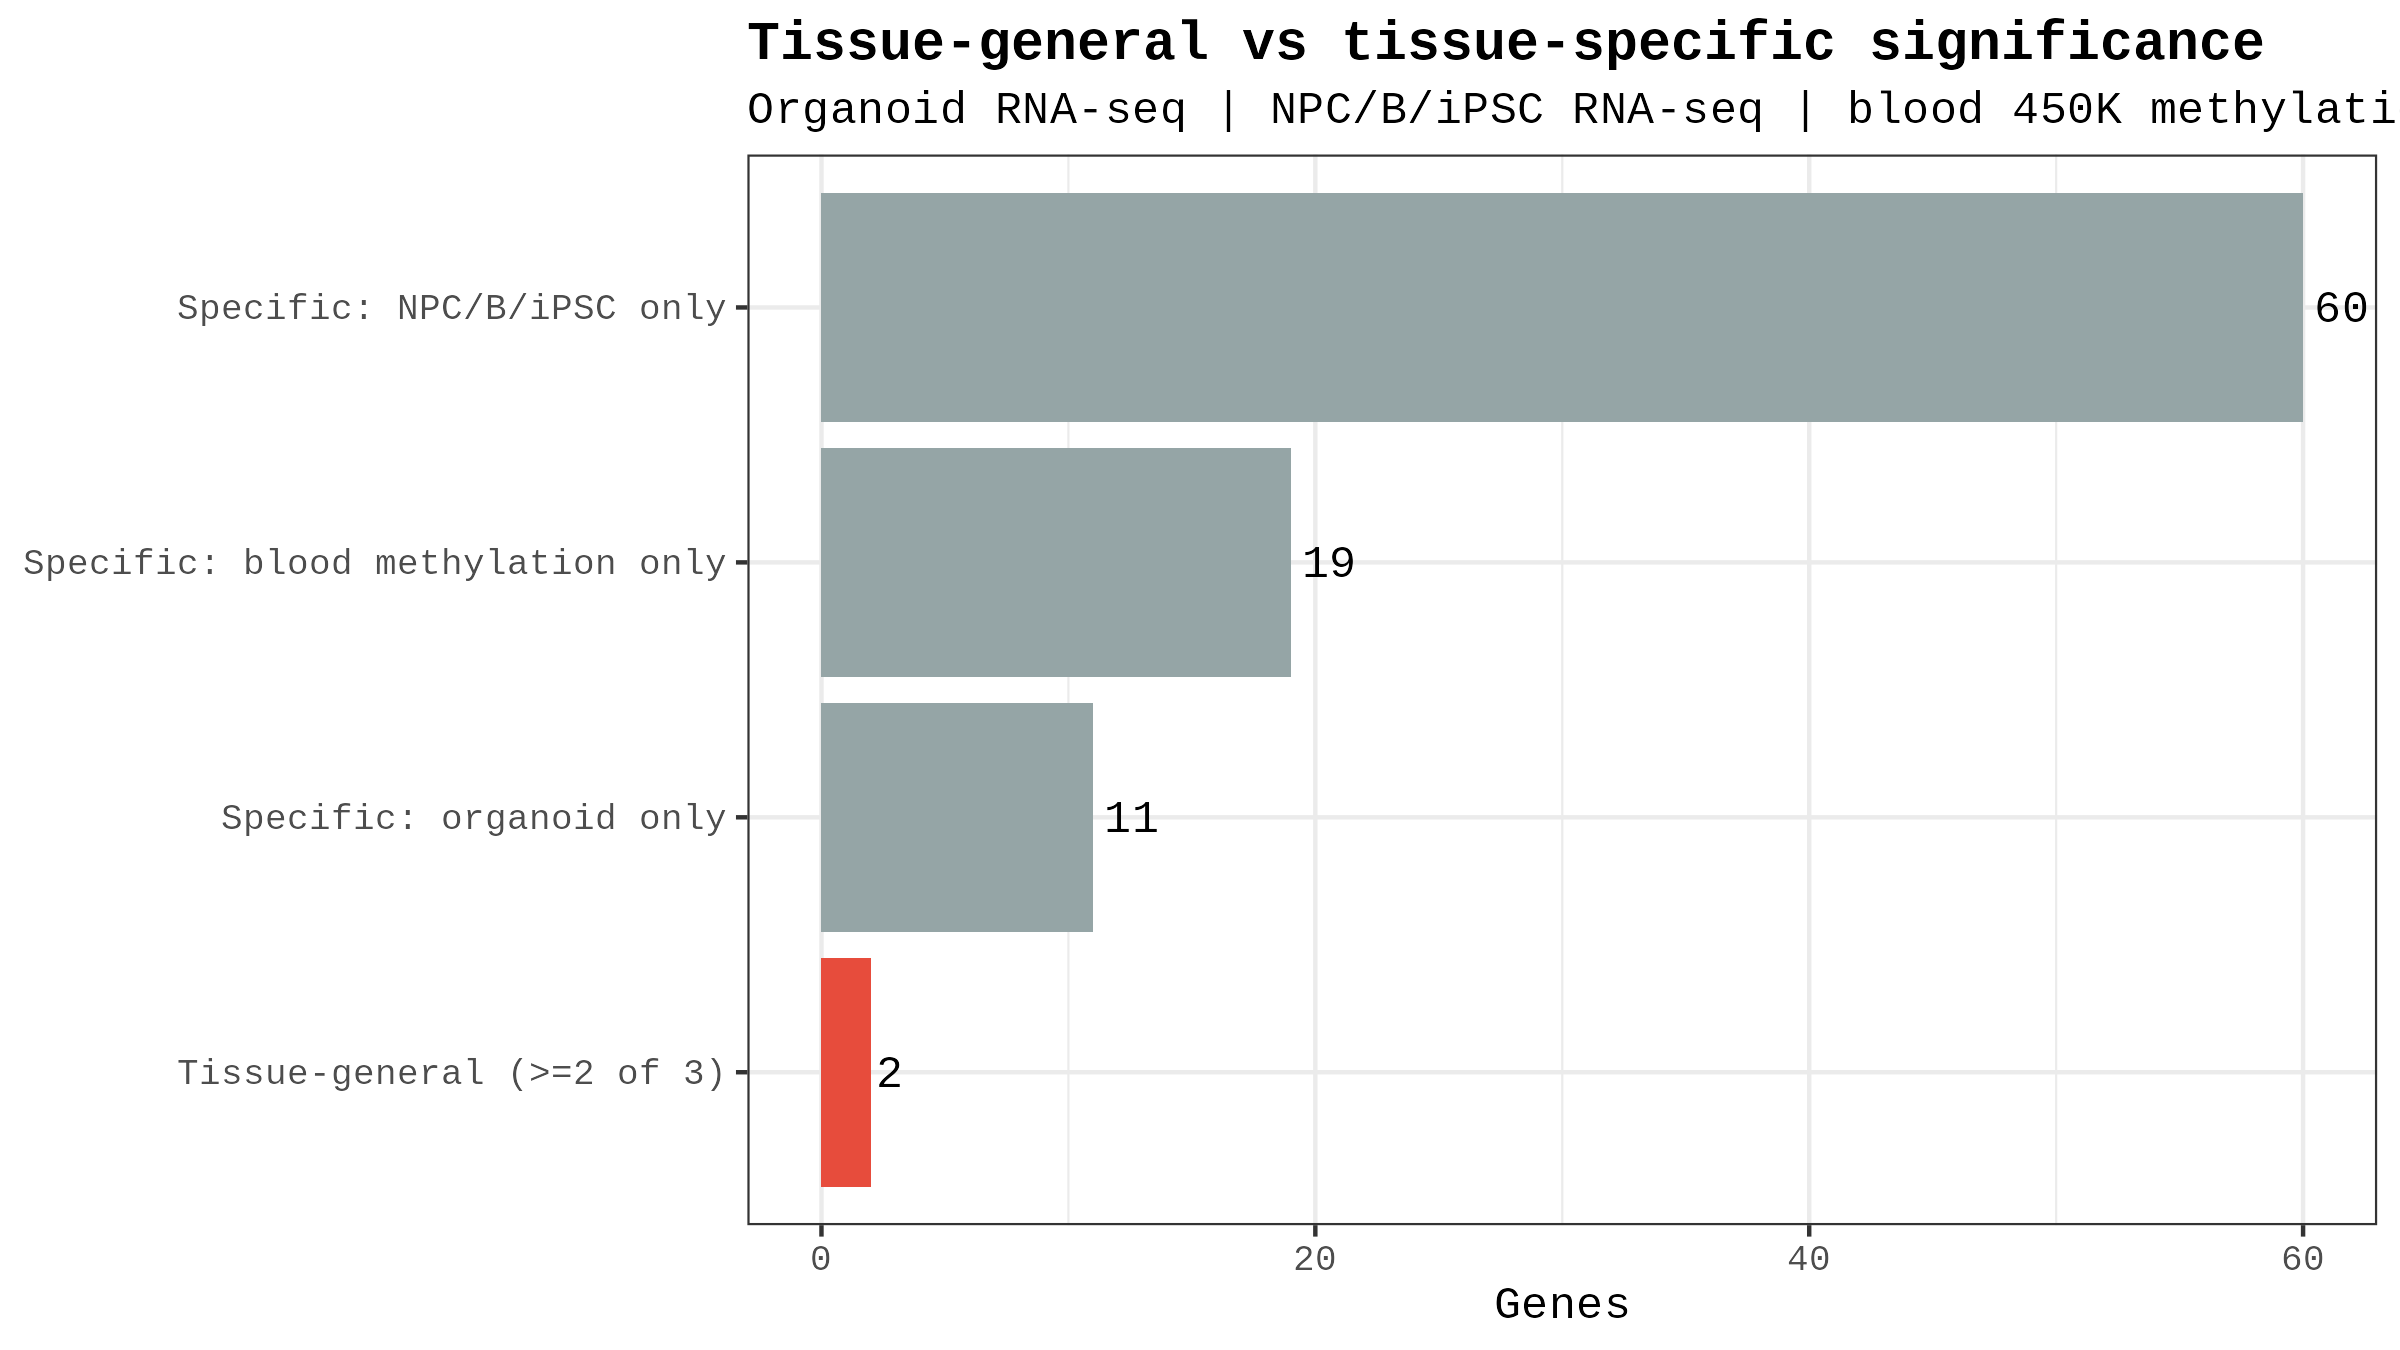
\includegraphics[width=0.9\columnwidth]{tissue_generality.png}
\caption{Tissue-generality classification across organoid RNA-seq, NPC/B-lymphocyte/iPSC RNA-seq and blood methylation. Tissue-general: \gene{FMR1}, \gene{FMR1-AS1}.}
\label{fig:tissue}
\end{figure}

\subsection{In Silico Regulator Validation}
ENCODE ChIP-seq self-recovery was evaluated for 22 TF--network pairs (11 TFs, GENIE3 and PANDA targets each). REST ranked first in ChEA3's ENCODE ChIP-seq library for both GENIE3- and PANDA-derived targets; SPI1, NRF1 and BHLHE40 (PANDA) ranked 2, 3 and 4, and MAZ (GENIE3) 7. Overall, 6 of 22 pairs ranked $\leq10$ and 8 ranked $\leq25$; SP1 ranked 53 (PANDA) and 96 (GENIE3), and TFAP2A 24 (PANDA) (Fig.~\ref{fig:encode}). Ranks in ChEA3's integrated score across all its libraries (1,632 TFs) were less extreme (REST 74 and 180), so the support is specific to direct-binding evidence.

In TRRUST, one of 24 pairs passed FDR: REST with GENIE3 targets ($4.6\times$ enrichment, 8 of 22 curated targets, FDR $=0.004$). REST with PANDA targets, SP1 with PANDA targets and TFAP2A with GENIE3 targets were nominally enriched only ($p=0.026$, $0.042$, $0.048$). CollecTRI, an independent and larger curated resource, gave the same result: REST with GENIE3 targets ($4.3\times$, 17 of 50 curated targets, FDR $=5.1\times10^{-6}$), with REST--PANDA nominally enriched ($p=0.005$, FDR $=0.11$).

\begin{figure}[!t]
\centering
\twofig{ChEA3_ENCODE_validation.png}{TRRUST_validation.png}
\caption{In silico validation. Left: ENCODE ChIP-seq self-recovery rank (green: rank $\leq10$). Right: fold enrichment of predicted targets among TRRUST curated targets (green: FDR $<0.05$).}
\label{fig:encode}
\end{figure}

TF activities inferred from CollecTRI regulons did not correlate between cohorts (737 TFs; Spearman $\rho=-0.019$, $p=0.60$; Fig.~\ref{fig:activity}); 38 TFs were significant in the organoids and 33 in the validation lines, and one in both: CTNNB1, reduced in FXS in each cohort (scores $-3.89$ and $-3.74$). Among reference TFs, SP1 activity was lower in FXS in both cohorts (organoid $-2.45$, FDR $=0.14$; validation $-4.39$, FDR $=0.003$), as was TFAP2A (validation FDR $=0.022$); SIX3 was reduced in organoids only (FDR $=0.003$), and REST activity did not change in either cohort.

\begin{figure}[!t]
\centering
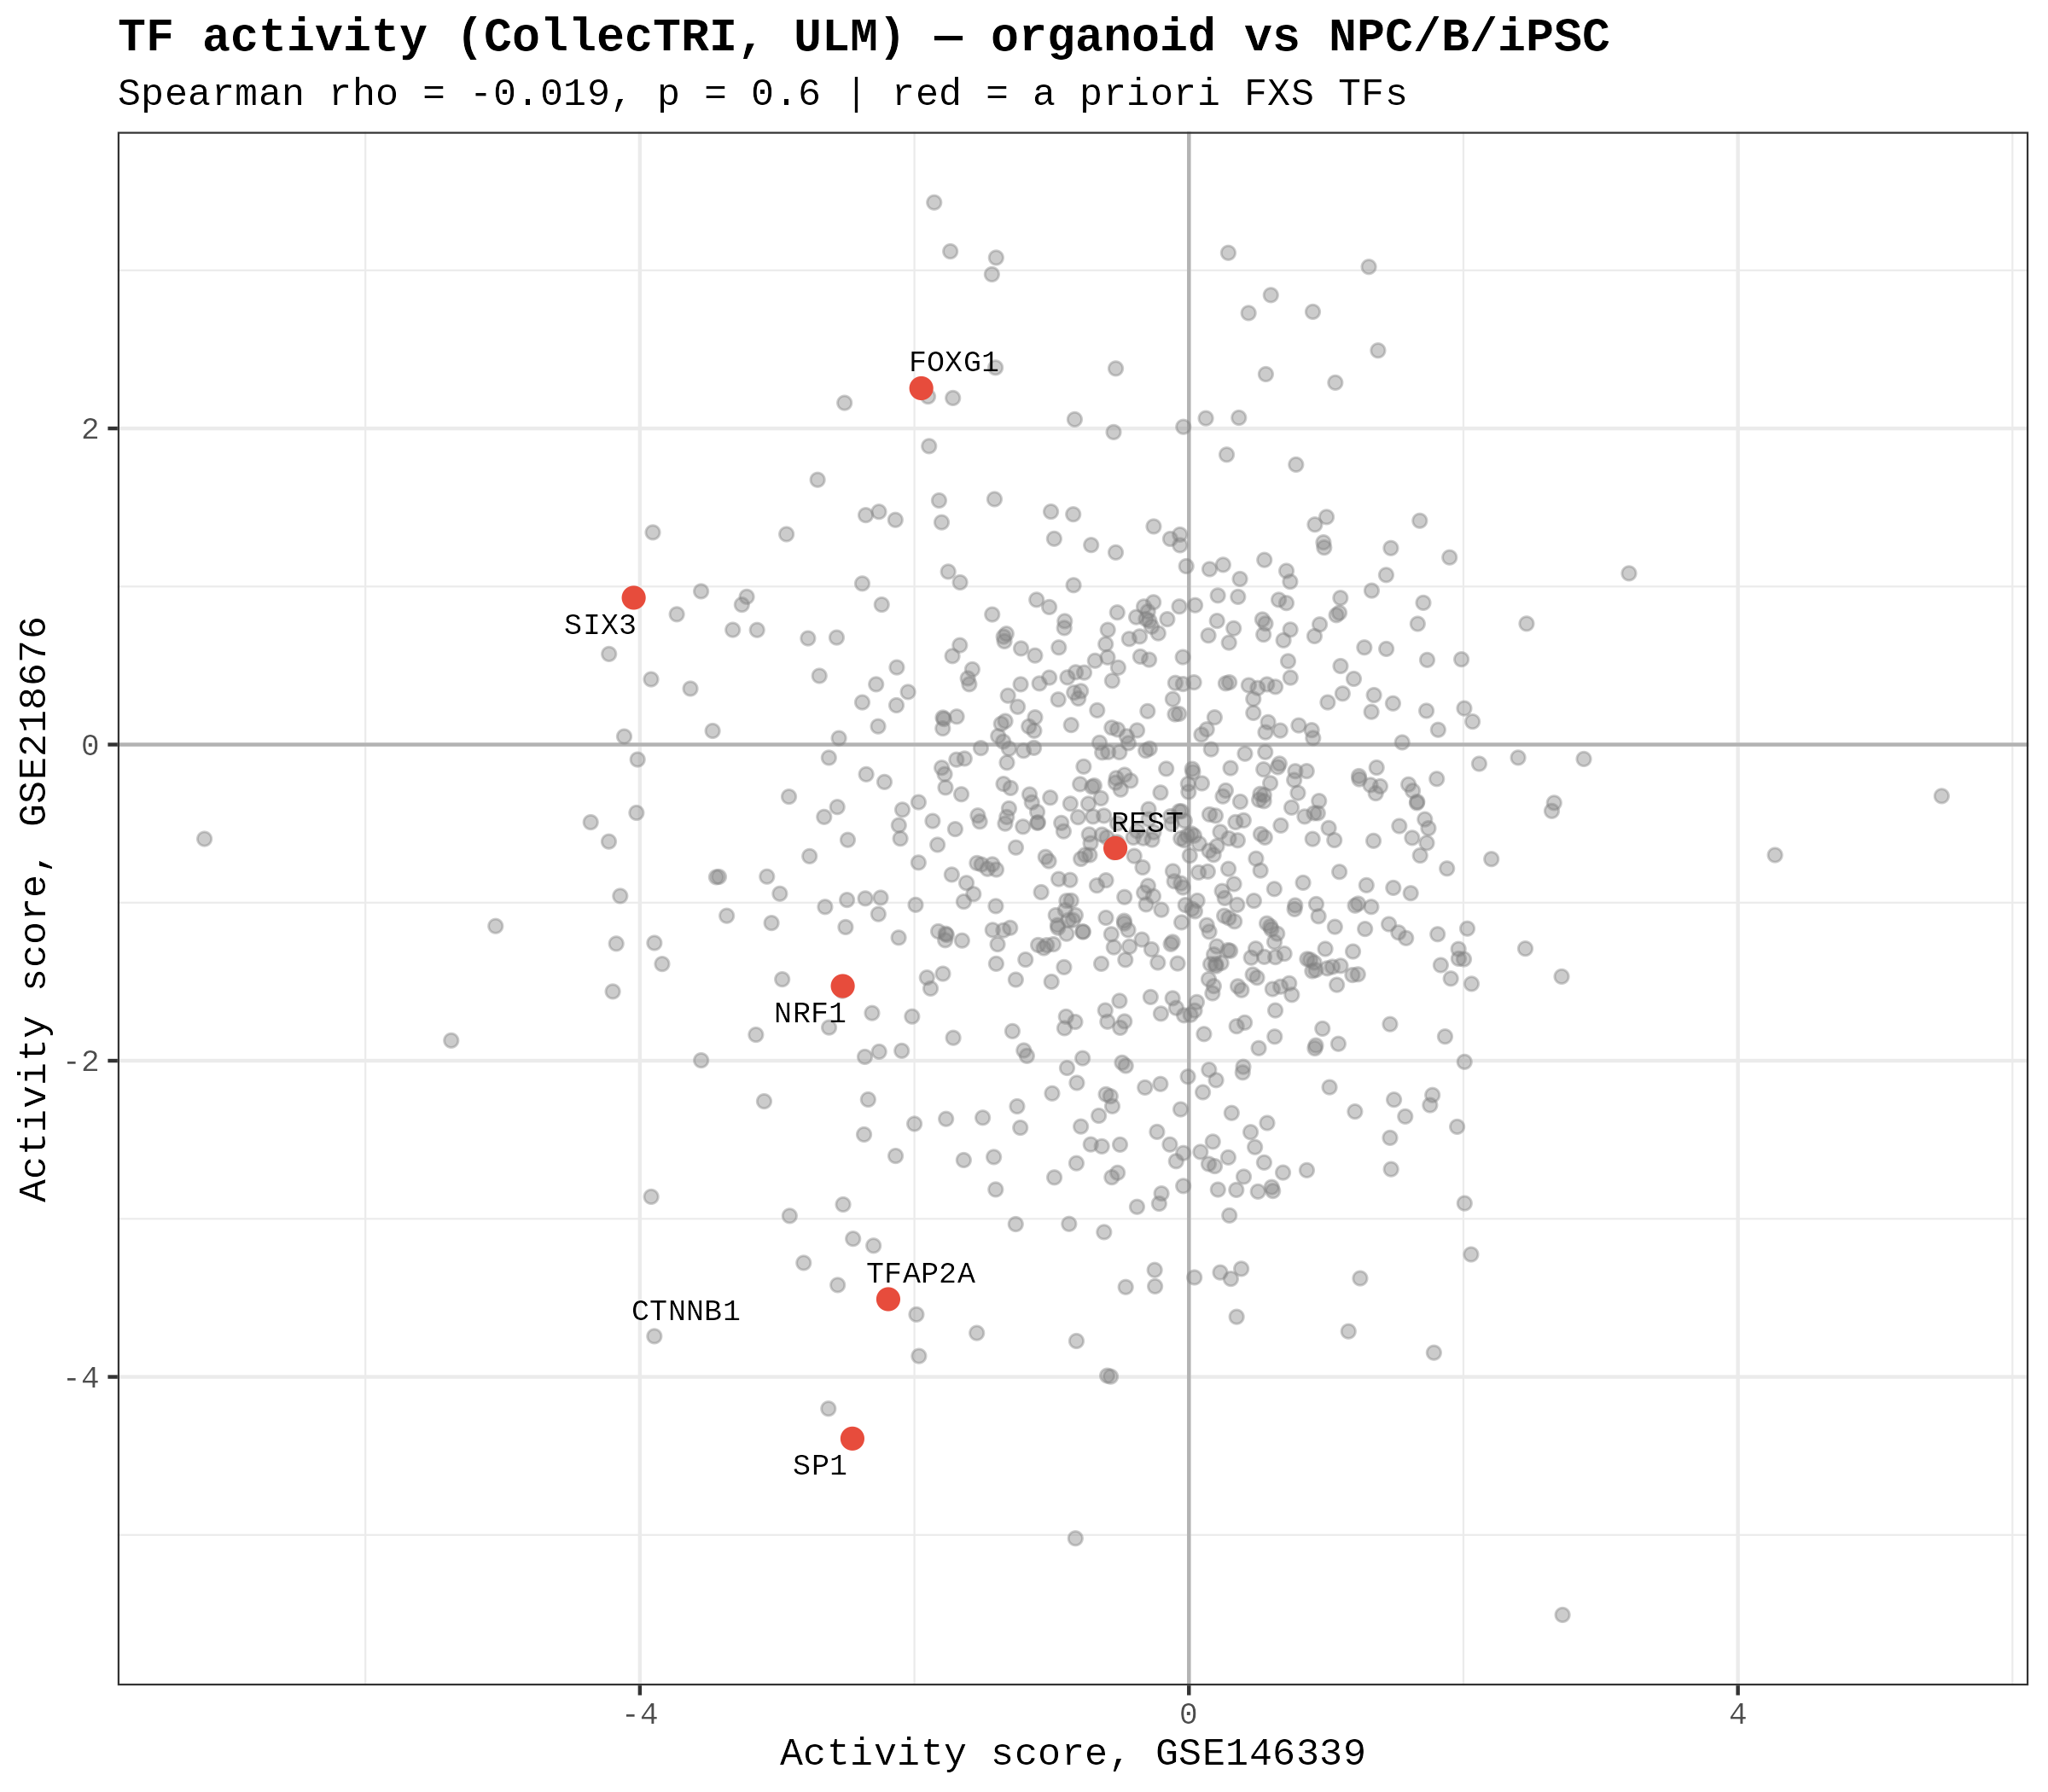
\includegraphics[width=0.92\columnwidth]{TF_activity_crosscohort.png}
\caption{TF activity (CollecTRI regulons, univariate linear model) in the organoid vs.\ validation cohort. Red: reference TFs; CTNNB1 is the only TF significant in both.}
\label{fig:activity}
\end{figure}

\begin{table*}[!t]
\centering
\caption{Supplementary materials. All paths are relative to \url{https://github.com/adj-04/fxs-research}.}
\label{tab:supp}
\small
\begin{tabular}{@{}>{\raggedright}p{0.05\textwidth}>{\raggedright}p{0.36\textwidth}p{0.52\textwidth}@{}}
\toprule
Item & Content & Repository file(s)\\
\midrule
S1 & Primary cohort DESeq2 results (13 DEGs) & \repo{results/DE/DESeq2_FXS_vs_Control_all.csv}, \repo{DESeq2_significant_DEGs.csv}\\
S2 & Validation cohort DE: DESeq2 (63 DEGs) and donor-blocked limma-voom & \repo{results/validation/GSE218676_validation_DEA_all.csv}, \repo{GSE218676_validation_limma_donorblock_all.csv}, \repo{validation_donor_sensitivity.csv}\\
S3 & Methylation: DMPs, gene summary, cell proportions, model comparison, \gene{FMR1} probes & \repo{results/methylation/DMP_FXS_vs_Control_significant.csv}, \repo{methylation_gene_summary.csv}, \repo{EpiDISH_cell_proportions.csv}, \repo{DMP_model_comparison.csv}, \repo{FMR1_probes_celltype_sensitivity.csv}\\
S4 & Promoter methylation per gene (PANDA prior weight) & \repo{results/methylation/promoter_methylation_by_gene.csv}\\
S5 & GENIE3 network, centrality, target universe, pooled-null summary & \repo{results/GENIE3/}\\
S6 & PANDA network, centrality, pooled-null summary & \repo{results/PANDA/}\\
S7 & LIONESS bootstrap and top limma-tested edges & \repo{results/LIONESS/}\\
S8 & ALPACA modules, node and module significance, local centrality, GO/KEGG & \repo{results/ALPACA/}\\
S9 & Cross-cohort concordance, overlap test, RRHO matrix & \repo{results/validation/crossvalidation_*.csv}, \repo{RRHO_manual_matrix.csv}\\
S10 & ENCODE (ChEA3), TRRUST and CollecTRI validation; TF activity & \repo{results/validation/}\\
S11 & Tissue-generality classification and pairwise tests & \repo{results/tissue_generality/}\\
S12 & Cytoscape network, style and session & \repo{networks/}\\
S13 & Scripts, Colab notebook, figures, logs, headline numbers & \repo{scripts/}, \repo{colab/}, \repo{figures/}, \repo{logs/}, \repo{results/v5_headline_numbers.csv}\\
\bottomrule
\end{tabular}
\end{table*}

\section{Discussion}
These results support a narrower and more specific claim than the framework was built to test. \gene{FMR1} silencing replicates across three datasets and three tissues, and its promoter hypermethylation is robust to blood-composition adjustment; this is expected for the causal lesion. What does not replicate is genome-wide regulatory rewiring: cross-cohort effect-size correlation is near zero with or without shrinkage, TF activities do not correlate between cohorts, no GENIE3, PANDA or LIONESS edge passes FDR, and PANDA's edge scores match its randomized-prior null. Unlike tests whose resolution makes significance impossible, these nulls could have detected edges at FDR $<0.05$, so their emptiness is informative: at $n=6$ versus $n=6$ the edge-level structure is not distinguishable from chance. Read with the tissue-generality classification, the weak correlation looks less like a pipeline failure than a finding: nearly every downstream effect is confined to one tissue context, and the \gene{FMR1} locus is the sole exception. We cannot fully separate this from limited power with two RNA-seq cohorts, but a near-zero genome-wide correlation is what a tissue-restricted picture predicts. The validation cohort adds a caution: once donor structure is modelled, its 63 line-level DEGs reduce to \gene{FMR1} alone, so the true number of tissue-specific changes is uncertain.

Beneath these negative results, two specific signals stand out. First, ALPACA module 4 is the only network structure that survives correction and remains significant with half the permutations. It joins BARHL1 and OTX1, homeobox TFs of neuronal specification and anterior brain patterning, with the neurofilament gene \gene{NEFL}, which fits a disorder of neuronal maturation studied in cerebral organoids. With five nodes and a single cohort, it is a concrete hypothesis to test rather than a mechanism. Second, REST has the most consistent support of the a priori regulators: its predicted targets rank REST first in ENCODE ChIP-seq enrichment for both network methods, are enriched among curated REST targets in two independent databases, and REST is among the top 30 GENIE3 hubs. REST (NRSF) represses neuronal genes in non-neuronal and progenitor cells, which makes its prominence in a neurodevelopmental model plausible. REST activity, however, did not differ between FXS and controls, so the evidence is that the networks recover REST's regulon correctly, not that REST is dysregulated in FXS. SP1 shows the converse pattern: weak network-level validation but reduced inferred activity in FXS in both cohorts, significant in the validation lines, and high local centrality alongside TFAP2A, NRF1 and REST in one module. CTNNB1, the only TF with significantly reduced activity in both cohorts, is consistent with the reduced Hedgehog-pathway genes (\gene{SHH}, \gene{GLI1}) among the organoid DEGs, but this too requires direct testing.

Local centrality alone does not single out these regulators: the module containing SP1, TFAP2A, NRF1 and REST is not itself differential, and FOXG1 is equally central without database support. Reporting the module- or hub-level findings without the nulls, the donor-blocked reanalysis, or the cell-composition adjustment would have overstated what these data support.

Finally, the significant RRHO peak alongside chance-level sign concordance is a general lesson for small-cohort genomics: rank-based overlap and aggregate correlation measure different things, and neither alone shows whether two cohorts agree. A second lesson is methodological: per-edge permutation nulls with tens of permutations cannot support FDR control over millions of edges, and should be replaced by pooled nulls or many more permutations.

\section{Limitations}
As with most network studies of rare disorders, the scope of these results is shaped mainly by the available data. The cohorts are small (six FXS and six control organoids; five lines per group in validation), so the absence of edge-level structure should be read as a statement about this scale rather than about FXS regulation in general. The three datasets come from different tissues and individuals, which enables the tissue-generality comparison but means a gene classed as tissue-specific may simply be under-detected elsewhere; for the same reason, methylation contributes a population-level prior rather than subject-matched integration, and age and array batch, which are not recorded for GSE41273, could not be modelled. Timepoint is handled as an additive effect, so FXS effects that differ between developmental stages are not captured, and the variance-ranked target universe may omit some low-variance targets. The pooled nulls assume comparable scores across edges and nodes, and module~4 rests on 20 permutations, although it was stable with 10. Finally, agreement with ENCODE, TRRUST and CollecTRI supports the plausibility of the inferred regulons; establishing causal roles in FXS will require experimental follow-up.

\section{Future Work}
The most direct next step is applying this framework to larger FXS cohorts as they become available. Single-cell and spatial transcriptomics would allow cell-type-specific rewiring to be resolved, matched multi-omic cohorts would allow methylation to enter at the subject level, and interaction models would capture timepoint-specific FXS effects. Methodologically, comparison with ARACNe and GRNBoost2 and sensitivity analyses across target-universe sizes and network thresholds would show how much of the reported structure is method-specific. Experimentally, module 4 (BARHL1, OTX1, \gene{NEFL}) and the REST and SP1 findings are the most specific candidates for perturbation (CRISPRi, reporter assays, ChIP) in FXS neural models.

\section{Conclusion}
We built a reproducible GRN framework for Fragile X syndrome that combines RNA-seq, cell-composition-adjusted methylation, GENIE3, PANDA, LIONESS and ALPACA with FDR-capable pooled permutation nulls, covariate-adjusted sample-specific networks, a second independent cohort, a tissue-generality classification and three-source in silico validation. \gene{FMR1} silencing replicates across all datasets, confirming known biology. Genome-wide regulatory rewiring does not clear significance at the sample sizes available, and downstream change is almost entirely tissue-restricted. Within that picture, one differential module linking BARHL1 and OTX1 to \gene{NEFL} survives correction, and REST emerges as the most consistently validated regulator, with SP1 showing reduced activity in FXS. We release the pipeline, a Colab notebook that reproduces it from public data, all result tables including negative results, and run logs as a template for regulatory network analysis in small rare-disease cohorts.

\section*{Data and Code Availability}
Raw data are public in NCBI GEO (GSE146339, GSE218676, GSE41273) and are fetched by \repo{scripts/01_fetch_data.R}. Code, result tables (including negative-result and permutation-null tables), network files, figures, Cytoscape style and session files, package versions and full run logs are at \url{https://github.com/adj-04/fxs-research}; \repo{colab/FXS_GRN_v5_Colab.ipynb} reproduces the analysis on Google Colab. Very large intermediate tables (complete GENIE3, PANDA and LIONESS edge lists) are regenerated by the scripts. Table~\ref{tab:supp} maps supplementary items to repository files.



\begin{thebibliography}{99}
\bibitem{santoro2012} M.~R. Santoro, S.~M. Bray, and S.~T. Warren, ``Molecular mechanisms of fragile X syndrome: A twenty-year perspective,'' \emph{Annu. Rev. Pathol.}, vol.~7, pp.~219--245, 2012.
\bibitem{peprah2012} E.~Peprah, ``Fragile X syndrome: The FMR1 CGG repeat distribution among world populations,'' \emph{Ann. Hum. Genet.}, vol.~76, no.~2, pp.~178--191, 2012.
\bibitem{hayward2021} B.~E. Hayward and K.~Usdin, ``Mechanisms of genome instability in the fragile X-related disorders,'' \emph{Genes}, vol.~12, no.~10, 2021.
\bibitem{li2020} M.~Li \emph{et al.}, ``Identification of FMR1-regulated molecular networks in human neurodevelopment,'' \emph{Genome Res.}, vol.~30, no.~3, 2020.
\bibitem{malachowski2023} T.~Malachowski, K.~R. Chandradoss, R.~Boya, \emph{et al.}, ``Spatially coordinated heterochromatinization of long synaptic genes in fragile X syndrome,'' \emph{Cell}, vol.~186, no.~26, pp.~5840--5858.e36, 2023.
\bibitem{liu2018} X.~S. Liu \emph{et al.}, ``Rescue of fragile X syndrome neurons by DNA methylation editing of the FMR1 gene,'' \emph{Cell}, vol.~172, no.~5, pp.~979--992, 2018.
\bibitem{brykczynska2016} U.~Brykczynska \emph{et al.}, ``CGG repeat-induced FMR1 silencing depends on the expansion size in human iPSCs and neurons carrying unmethylated full mutations,'' \emph{Stem Cell Rep.}, vol.~7, no.~6, pp.~1059--1071, 2016.
\bibitem{boland2017} M.~J. Boland \emph{et al.}, ``Molecular analyses of neurogenic defects in a human pluripotent stem cell model of fragile X syndrome,'' \emph{Brain}, vol.~140, no.~3, pp.~582--598, 2017.
\bibitem{lu2016} P.~Lu \emph{et al.}, ``Integrated transcriptome analysis of human iPS cells derived from a fragile X syndrome patient during neuronal differentiation,'' \emph{Sci. China Life Sci.}, vol.~59, no.~11, 2016.
\bibitem{rogers2017} T.~D. Rogers \emph{et al.}, ``Effects of a social stimulus on gene expression in a mouse model of fragile X syndrome,'' \emph{Mol. Autism}, vol.~8, 2017.
\bibitem{arsenault2021} J.~Arsenault \emph{et al.}, ``Interregulation between fragile X mental retardation protein and methyl CpG binding protein 2 in the mouse posterior cerebral cortex,'' \emph{Hum. Mol. Genet.}, vol.~30, no.~16, 2021.
\bibitem{nitsch2009} D.~Nitsch \emph{et al.}, ``Network analysis of differential expression for the identification of disease-causing genes,'' \emph{PLoS ONE}, vol.~4, no.~5, e5526, 2009.
\bibitem{davidovic2011} L.~Davidovic \emph{et al.}, ``A metabolomic and systems biology perspective on the brain of the fragile X syndrome mouse model,'' \emph{Genome Res.}, vol.~21, no.~12, pp.~2190--2202, 2011.
\bibitem{genie3} V.~A. Huynh-Thu, A.~Irrthum, L.~Wehenkel, and P.~Geurts, ``Inferring regulatory networks from expression data using tree-based methods,'' \emph{PLoS ONE}, vol.~5, no.~9, e12776, 2010.
\bibitem{panda} K.~Glass, C.~Huttenhower, J.~Quackenbush, and G.-C. Yuan, ``Passing messages between biological networks to refine predicted interactions,'' \emph{PLoS ONE}, vol.~8, no.~5, e64832, 2013.
\bibitem{lioness} M.~L. Kuijjer, M.~G. Tung, G.~Yuan, J.~Quackenbush, and K.~Glass, ``Estimating sample-specific regulatory networks,'' \emph{iScience}, vol.~14, pp.~226--240, 2019.
\bibitem{alpaca} M.~Padi and J.~Quackenbush, ``Detecting phenotype-driven transitions in regulatory network structure,'' \emph{npj Syst. Biol. Appl.}, vol.~4, 16, 2018.
\bibitem{netzoo} M.~Ben~Guebila \emph{et al.}, ``The Network Zoo: A multilingual package for the inference and analysis of gene regulatory networks,'' \emph{Genome Biol.}, vol.~24, 45, 2023.
\bibitem{string2023} D.~Szklarczyk \emph{et al.}, ``The STRING database in 2023: Protein--protein association networks and functional enrichment analyses for any sequenced genome of interest,'' \emph{Nucleic Acids Res.}, vol.~51, no.~D1, pp.~D638--D646, 2023.
\bibitem{jaspar2020} O.~Fornes \emph{et al.}, ``JASPAR 2020: Update of the open-access database of transcription factor binding profiles,'' \emph{Nucleic Acids Res.}, vol.~48, no.~D1, pp.~D87--D92, 2020.
\bibitem{deseq2} M.~I. Love, W.~Huber, and S.~Anders, ``Moderated estimation of fold change and dispersion for RNA-seq data with DESeq2,'' \emph{Genome Biol.}, vol.~15, 550, 2014.
\bibitem{apeglm} A.~Zhu, J.~G. Ibrahim, and M.~I. Love, ``Heavy-tailed prior distributions for sequence count data: Removing the noise and preserving large differences,'' \emph{Bioinformatics}, vol.~35, no.~12, pp.~2084--2092, 2019.
\bibitem{voom} C.~W. Law, Y.~Chen, W.~Shi, and G.~K. Smyth, ``voom: Precision weights unlock linear model analysis tools for RNA-seq read counts,'' \emph{Genome Biol.}, vol.~15, R29, 2014.
\bibitem{dupcor} G.~K. Smyth, J.~Michaud, and H.~S. Scott, ``Use of within-array replicate spots for assessing differential expression in microarray experiments,'' \emph{Bioinformatics}, vol.~21, no.~9, pp.~2067--2075, 2005.
\bibitem{limma} M.~E. Ritchie, B.~Phipson, D.~Wu, Y.~Hu, C.~W. Law, W.~Shi, and G.~K. Smyth, ``limma powers differential expression analyses for RNA-sequencing and microarray studies,'' \emph{Nucleic Acids Res.}, vol.~43, no.~7, e47, 2015.
\bibitem{epidish} A.~E. Teschendorff, C.~E. Breeze, S.~C. Zheng, and S.~Beck, ``A comparison of reference-based algorithms for correcting cell-type heterogeneity in epigenome-wide association studies,'' \emph{BMC Bioinformatics}, vol.~18, 105, 2017.
\bibitem{minfi} M.~J. Aryee \emph{et al.}, ``Minfi: A flexible and comprehensive Bioconductor package for the analysis of Infinium DNA methylation microarrays,'' \emph{Bioinformatics}, vol.~30, no.~10, pp.~1363--1369, 2014.
\bibitem{clusterprofiler} G.~Yu, L.-G. Wang, Y.~Han, and Q.-Y. He, ``clusterProfiler: An R package for comparing biological themes among gene clusters,'' \emph{OMICS}, vol.~16, no.~5, pp.~284--287, 2012.
\bibitem{cytoscape} P.~Shannon \emph{et al.}, ``Cytoscape: A software environment for integrated models of biomolecular interaction networks,'' \emph{Genome Res.}, vol.~13, no.~11, pp.~2498--2504, 2003.
\bibitem{rcy3} J.~A. Gustavsen, S.~Pai, R.~Isserlin, B.~Demchak, and A.~R. Pico, ``RCy3: Network biology using Cytoscape from within R,'' \emph{F1000Research}, vol.~8, 1774, 2019.
\bibitem{rrho} S.~B. Plaisier, R.~Taschereau, J.~A. Wong, and T.~G. Graeber, ``Rank--rank hypergeometric overlap: Identification of statistically significant overlap between gene-expression signatures,'' \emph{Nucleic Acids Res.}, vol.~38, no.~17, e169, 2010.
\bibitem{chea3} A.~B. Keenan \emph{et al.}, ``ChEA3: Transcription factor enrichment analysis by orthogonal omics integration,'' \emph{Nucleic Acids Res.}, vol.~47, no.~W1, pp.~W212--W224, 2019.
\bibitem{encode2012} The ENCODE Project Consortium, ``An integrated encyclopedia of DNA elements in the human genome,'' \emph{Nature}, vol.~489, pp.~57--74, 2012.
\bibitem{trrust} H.~Han \emph{et al.}, ``TRRUST v2: An expanded reference database of human and mouse transcriptional regulatory interactions,'' \emph{Nucleic Acids Res.}, vol.~46, no.~D1, pp.~D380--D386, 2018.
\bibitem{collectri} S.~M\"uller-Dott \emph{et al.}, ``Expanding the coverage of regulons from high-confidence prior knowledge for accurate estimation of transcription factor activities,'' \emph{Nucleic Acids Res.}, vol.~51, no.~20, pp.~10934--10949, 2023.
\bibitem{decoupler} P.~Badia-i-Mompel \emph{et al.}, ``decoupleR: Ensemble of computational methods to infer biological activities from omics data,'' \emph{Bioinform. Adv.}, vol.~2, no.~1, vbac016, 2022.
\end{thebibliography}

\end{document}
